\section{Case study: the minivan (Petrin 2002)}\label{sec:10-petrin}

\citet{Petrin2002} measures the welfare created by the minivan, a vehicle that Chrysler introduced in 1984 and that
its rivals imitated within two years. The paper answers two questions. The first is substantive. How large were the
gains to consumers and to each producer, and how were they shared? The second is methodological. How can a
researcher who has only market-level data discipline the random coefficients that govern substitution, and therefore
welfare? Petrin's answer to the second question, the use of \emph{micro moments}, is now a standard part of demand
estimation (\cref{sec:08-micro-moments}). \Cref{tab:10-petrin-map} at the end of the section maps the study.
We follow the paper from its question to its contribution, as in
\cref{sec:10-hausman}.\footnote{Petrin writes $\gamma_k$ for the scale of the random coefficient on characteristic $k$,
$\gamma_{mi}$, $\gamma_{sw}$, $\gamma_{su}$ and $\gamma_{pv}$ for the family-vehicle interactions, and $\tau$ for the
cost parameters. In his text the income-group price coefficients are $\alpha_0$, $\alpha_1$ and $\alpha_2$, while his
Table 4 labels them $\alpha_1$, $\alpha_2$ and $\alpha_3$. We write $\sigma_k$, $\pi_{\mathrm{mv}}$, $\pi_{\mathrm{sw}}$,
$\pi_{\mathrm{su}}$, $\pi_{\mathrm{pv}}$ and $\gamma$, and we follow the table for the price coefficients. Page and
table numbers in this section refer to the journal article.}

\subsection{The question}\label{sec:10-petrin-question}

New products improve the standard of living, and firms introduce them to earn the temporary market power of a first
mover (p.~705). Petrin estimates three objects for the minivan. The first is the compensating variation of consumers,
including the gains of households that bought other vehicles whose prices fell when the minivan arrived. The second
is the change in producer surplus. It combines Chrysler's first-mover profits, the cannibalization of its own station
wagons, and the losses imposed on Ford and General Motors (GM). The third is the profit that the imitators dissipated
when they entered.

The question matters for the theory of \cref{sec:10-imperfect}. There we saw that a new good changes welfare through
the surplus of its own buyers and through the prices of existing goods. \Cref{tab:10-bresnahan-2x2} called the second
channel ``Competition,'' and \cref{sec:10-bresnahan} criticized \citet{Hausman1997} for holding rivals' prices fixed.
Petrin re-solves the pricing equilibrium of the whole automobile market with and without minivans. His estimates
therefore measure the Competition cell, together with Chrysler's repricing of its own wagons, in one equilibrium
calculation.

The method matters as much as the answer. Random coefficients are imprecisely estimated from market shares alone
(\cref{sec:08-instruments}). Welfare numbers inherit that imprecision, and they inherit the dependence on the
idiosyncratic logit shock described in \cref{sec:10-charspace}. Petrin's abstract states the main finding in these
terms. Models estimated without micro data yield much larger welfare numbers, ``primarily because the micro data
appear to free the model from a heavy dependence on the idiosyncratic logit `taste' error'' (p.~705).

\subsection{The minivan innovation}\label{sec:10-petrin-setting}

Ford proposed a vehicle called the ``Mini/Max'' in the early 1970s (p.~707). It was a boxlike vehicle that obtained
interior space from its height, with front-wheel drive that lowered the passenger floor. Ford's management gave the
idea little support because it feared cannibalizing the firm's strong station wagon sales. This is the private
incentive problem of \cref{sec:10-imperfect} in its purest form. A firm that owns close substitutes values a new
product only net of the profits it diverts from them.

The financially troubled Chrysler Corporation introduced the Dodge Caravan in 1984. It sold 170,000 units in its first
year. GM introduced the Astro and Safari in 1985, and Ford introduced the Aerostar in 1986. Both rivals were unprepared
for the Caravan's success. They built their minivans on truck platforms with rear-wheel drive, so these vehicles
handled more like downsized full-size vans than like passenger cars. Chrysler kept its lead by adding a larger engine
and a second sliding door. Fourteen years after the introduction, six firms sold 13 minivans, and Chrysler held 44
percent of a market of 1.16 million vehicles. Station wagon sales peaked at 950,000 in 1984 and fell to 300,000 over
the next seven years (p.~707).

Table~3 of the paper shows the substitution in shares of total vehicle sales. Minivans rose from 1.58 percent in 1984 to
9.93 percent in 1993. Station wagons held about 10 percent in 1981--83 (10.51, 10.27 and 10.32 percent), fell to 8.90
percent in 1984, and reached 3.02 percent in 1993. The combined share of minivans and wagons stayed between 9.65 and
12.95 percent over 1981--93. Petrin reads this negative comovement as evidence of a positive covariance in the tastes
for the two vehicle types (p.~718). The demand model is built to capture that covariance.

\subsection{Data}\label{sec:10-petrin-data}

The paper combines two data sets (pp.~712--713). The market data cover all 2,407 nameplates sold in the United States
from 1981 to 1993 with annual sales above 1,000 vehicles. They come from the \textit{Automotive News Market Data
Book} and \textit{Ward's Automotive Yearbook}. The characteristics are acceleration (horsepower per unit of curb
weight), size (length times width times height), drive type, fuel efficiency (miles per dollar), and a luxury proxy
(air conditioning standard). Quantity and list price refer to the base model. Nameplates in adjacent years whose
horsepower, wheelbase, width and length change by less than 10 percent are treated as the same model. This rule leaves
916 independent observations, and the standard errors allow arbitrary correlation of the errors of the same model over
time (p.~716, n.~11).

The consumer data come from the Consumer Expenditure Survey (CEX) for 1987--92. Almost 30,000 household records
approximate the joint distribution of demographics in the United States. The CEX automobile supplement links the
demographics of 2,660 new-vehicle buyers to the vehicles they bought. Among them are 120 minivan buyers, 63 station
wagon buyers, 131 sport-utility buyers and 23 full-size van buyers. These samples are too small for a consumer-level
choice model, since about 200 kinds of vehicles are sold each year but only about 400 purchases are recorded annually
(p.~713, n.~8). They are large enough to estimate a few averages precisely. Other annual inputs are the number of
households $M$, gasoline prices and the growth of gross national product. The random coefficients model without micro
data also uses a lognormal income distribution estimated from the March Current Population Survey (p.~713, n.~9).

\Cref{tab:10-petrin-cex} reproduces the demographic averages of Table~2 of the paper. They are the targets of the micro
moments. New-vehicle buyers had a mean income of \$36,113, about \$13,000 above the U.S. mean of \$23,728 (incomes
in 1982--84 dollars). Minivan buyers had the largest families of all buyer groups, 3.86 members against 2.58 in the
population. They also had the highest share of household heads aged 30 to 60, 78 percent against 55 percent. Table~1 of
the paper adds that minivans were larger than the average vehicle (size 0.87 against 0.71). Of them, 78 percent had air
conditioning as standard (27 percent of all vehicles), and their mean list price was \$10,060 against \$9,867 for all
vehicles. Chrysler accounted almost entirely for the 63 percent of minivan sales with front-wheel drive (p.~716).

\begin{table}[htbp]
\centering
\caption{Demographics of the U.S. population and of new-vehicle buyers, 1987--92}\label{tab:10-petrin-cex}
\small
\setlength{\tabcolsep}{5pt}
\begin{tabular}{@{}lccccccc@{}}
\toprule
 & \multicolumn{2}{c}{United States} & \multicolumn{5}{c}{Buyers of} \\
\cmidrule(lr){2-3}\cmidrule(l){4-8}
 & Mean & Std.\ dev. & New vehicles & Minivans & Wagons & Sport-utilities & Full-size vans \\
\midrule
Income (\$)  & 23,728 & 21,255 & 36,113 & 39,476 & 40,196 & 41,569 & 31,164 \\
Family size  & 2.58   & 1.53   & 2.87   & 3.86   & 3.17   & 2.97   & 3.47   \\
Midage       & 0.55   & 0.49   & 0.64   & 0.78   & 0.73   & 0.74   & 0.65   \\
\bottomrule
\end{tabular}

\smallskip
\begin{minipage}{0.95\textwidth}
\footnotesize Source: \citet[Table~2]{Petrin2002}, from the Consumer Expenditure Survey. Income is in 1982--84
CPI-adjusted dollars. Family size is the number of household members. Midage is an indicator for a household head
aged between 30 and 60 inclusive.
\end{minipage}
\end{table}

\subsection{The demand model}\label{sec:10-petrin-model}

Consumers are households $i$ with income $y_i$, family size $fs_i$, an indicator $\mathit{mid}_i$ for a head aged 30 to
60, and unobserved tastes. Each household buys one new vehicle $j \in \{1, \dots, J\}$ in a year or buys none ($j = 0$).
Petrin specifies the conditional indirect utility (p.~710)
\begin{equation}\label{eq:10-petrin-utility}
  u_{ij} = \alpha_i \ln(y_i - p_j) + x_j\beta + \sum_{k} \sigma_k \nu_{ik} x_{jk}
           + \ln(fs_i)\,\nu_{i,\mathrm{fv}} \sum_{g \in \mathcal{G}} \pi_g d_{jg} + \xi_j + \epsilon_{ij},
  \qquad j = 1, \dots, J .
\end{equation}
The first term is the utility of the composite good bought with the income left after the vehicle. The row vector
$x_j$ holds a constant, the five characteristics, four vehicle-type dummies, the percentage change in gross national
product and a quadratic time trend (Table~4, note). The set $\mathcal{G} = \{\mathrm{mv}, \mathrm{sw}, \mathrm{su},
\mathrm{pv}\}$ collects the four \emph{family vehicle} types: minivans, station wagons, sport-utility vehicles and
full-size passenger vans. The dummy $d_{jg}$ equals one when vehicle $j$ is of type $g$. The unobserved product quality
is $\xi_j$, and $\epsilon_{ij}$ is type-I extreme value.

Three features of \eqref{eq:10-petrin-utility} carry the economics.

\casehead{Income effects} The marginal utility of income varies across the three income terciles,
\begin{equation*}
  \alpha_i = \begin{cases}
    \alpha_1 & \text{if } y_i < \bar y_1, \\
    \alpha_2 & \text{if } \bar y_1 \le y_i < \bar y_2, \\
    \alpha_3 & \text{if } y_i \ge \bar y_2,
  \end{cases}
\end{equation*}
where $\bar y_1$ and $\bar y_2$ split the population into three equal groups. The utility cost of a higher price is
\begin{equation}\label{eq:10-petrin-dudp}
  \frac{\partial u_{ij}}{\partial p_j} = -\frac{\alpha_i}{y_i - p_j} ,
\end{equation}
so price sensitivity falls with income within a group, and the three $\alpha_g$ let the curvature differ across groups.
This is the Cobb-Douglas income specification of \citet{BerryLevinsohnPakes1995} studied in \cref{sec:08-income}, with
group-specific coefficients. Conditional on all tastes, the logit formulas give the individual share derivatives
\begin{equation*}
  \frac{\partial s_{ij}}{\partial p_j} = -\frac{\alpha_i}{y_i - p_j}\,s_{ij}(1 - s_{ij}), \qquad
  \frac{\partial s_{ij}}{\partial p_k} = \frac{\alpha_i}{y_i - p_k}\,s_{ij}s_{ik} \quad (k \ne j).
\end{equation*}
Market derivatives integrate these over households.

\casehead{Random tastes for characteristics} Household $i$ draws a taste $\nu_{ik}$ for each characteristic $k$,
scaled by $\sigma_k$. Petrin draws the $\nu_{ik}$ independently from a $\chi^2(3)$ distribution truncated at its 95th
percentile (p.~711). He gives two reasons. The distribution is bounded above and below, and it skews heterogeneity in
the direction of positive taste. Taken as written, the draws lie between 0 and 7.81, with mean about 2.63 and standard
deviation about 1.83 (our computation). The paper does not say whether the draws are \emph{centered}, that is, whether
their mean is subtracted before they enter utility. The random coefficient on the constant makes the value of buying any new vehicle,
relative to the outside option, heterogeneous across households.

\casehead{Demographic tastes for family vehicles} The taste of household $i$ for a family vehicle of type $g$ is
$\pi_g \ln(fs_i)\,\nu_{i,\mathrm{fv}}$. The draw $\nu_{i,\mathrm{fv}}$ is common to all four types, and family size
scales it. Conditional on family size, the covariance between the tastes for minivans and for station wagons is
\begin{equation}\label{eq:10-petrin-cov}
  \Cov\bigl(\pi_{\mathrm{mv}}\ln(fs_i)\nu_{i,\mathrm{fv}},\; \pi_{\mathrm{sw}}\ln(fs_i)\nu_{i,\mathrm{fv}} \bigm| fs_i\bigr)
  = \pi_{\mathrm{mv}}\pi_{\mathrm{sw}}\,\bigl(\ln fs_i\bigr)^2\,\Var(\nu_{i,\mathrm{fv}}) .
\end{equation}
It rises with $\pi_{\mathrm{mv}}$ and $\pi_{\mathrm{sw}}$ and with family size. Substitution between minivans and
wagons can therefore arise for two reasons (p.~710). Large families prefer both types, or the two types share other
observed characteristics such as size.

The outside option is to buy no new vehicle. We write its utility as $u_{i0} = \alpha_i\ln y_i + \epsilon_{i0}$, the
normalization of \cref{sec:08-income}. Conditional on the household's demographics $D_i = (y_i, fs_i, \mathit{mid}_i)$
and tastes $\nu_i$, the probability of buying $j$ is the logit formula (p.~711)
\begin{equation}\label{eq:10-petrin-sij}
  s_{ij} = \frac{\exp V_{ij}}{\exp\bigl(\alpha_i \ln y_i\bigr) + \sum_{l=1}^{J} \exp V_{il}} ,\qquad
  V_{ij} = \alpha_i\ln(y_i - p_j) + \delta_j + \mu_{ij},
\end{equation}
with base utility $\delta_j = x_j\beta + \xi_j$ and household-specific term
\begin{equation*}
  \mu_{ij} = \sum_k\sigma_k\nu_{ik}x_{jk} + \ln(fs_i)\,\nu_{i,\mathrm{fv}}\sum_g \pi_g d_{jg} .
\end{equation*}
Price is not part of $\delta_j$. It enters only through the income
term, so the $\alpha_g$ are nonlinear parameters, as in \cref{sec:08-income}. The market share is $s_j = \int s_{ij}\,
\dd P(D_i, \nu_i)$, where $D_i$ follows the empirical distribution of the CEX and $\nu_i$ the truncated $\chi^2(3)$
distribution. Petrin calls the elements of $\beta$ \emph{base coefficients} (Table~4). If the draws are centered,
$\mu_{ij}$ has mean zero and $\delta_j$ is the mean utility of product $j$, net of the income term. Otherwise
$\delta_j$ is that utility for a household whose draws are all zero, and the mean taste for characteristic $k$ is
$\beta_k + 2.63\,\sigma_k$.

The demand side has 24 parameters: three price coefficients, eleven base coefficients, six random-coefficient scales
and four family-vehicle interactions. Eleven of them describe family vehicles and income effects: the three
$\alpha_g$, the four type dummies and the four $\pi_g$. The micro moments speak most directly to these eleven.

\subsection{Supply and the counterfactual equilibrium}\label{sec:10-petrin-supply}

The supply side follows \citet{BerryLevinsohnPakes1995} (pp.~711--712). Multiproduct firms $f = 1, \dots, F$ set prices
in a static Bertrand-Nash equilibrium. Marginal cost is log-linear in observed cost characteristics $W_j$ and an
unobserved component $\omega_j$,
\begin{equation}\label{eq:10-petrin-mc}
  \ln mc_j = W_j\gamma + \omega_j .
\end{equation}
Firm $f$ earns $\Pi_f = M\sum_{j\in\mathcal{J}_f}(p_j - mc_j)\,s_j(p, x; \theta)$, and the first-order conditions are
\begin{equation}\label{eq:10-petrin-foc}
  s_j(p, x; \theta) + \sum_{r \in \mathcal{J}_f}(p_r - mc_r)\frac{\partial s_r(p, x; \theta)}{\partial p_j} = 0,
  \qquad j \in \mathcal{J}_f .
\end{equation}
In matrix form these are \eqref{eq:08-foc-matrix}, and inverting them gives the markup formula \eqref{eq:08-markup},
$p - mc = -[(\Omega\odot\Delta)^\top]^{-1}s$. Given demand estimates and observed prices, this formula recovers each
$mc_j$ \citep[eq.~3]{Petrin2002}.

A rearrangement of \eqref{eq:10-petrin-foc} is useful for reading the counterfactual. Separate the own-product term
and divide by $-\frac{\partial s_j}{\partial p_j} > 0$:
\begin{align}
  0 &= s_j + (p_j - mc_j)\frac{\partial s_j}{\partial p_j}
       + \sum_{r\in\mathcal{J}_f,\, r\ne j}(p_r - mc_r)\frac{\partial s_r}{\partial p_j}, \notag\\
  p_j - mc_j &= \frac{s_j}{-\frac{\partial s_j}{\partial p_j}}
       + \sum_{r\in\mathcal{J}_f,\, r\ne j}(p_r - mc_r)\,D_{jr},
  \qquad D_{jr} = \frac{\frac{\partial s_r}{\partial p_j}}{-\frac{\partial s_j}{\partial p_j}} . \label{eq:10-petrin-diversion}
\end{align}
Here $D_{jr}$ is the diversion ratio from $j$ to $r$ (\cref{ch:diffprod}). The markup on $j$ is a single-product
markup plus the margins the firm earns on the sales that a higher $p_j$ diverts to its other products. When Chrysler
adds a minivan $m$ that is a substitute for its station wagons, a new positive term $(p_m - mc_m)D_{jm}$ appears in the
markup of each Chrysler wagon $j$. Other things equal, Chrysler raises the prices of its wagons. Rival firms gain no
term for the minivan. Their markups change through the first term, which falls when entry makes their demand more
elastic, and through changes in diversion among their own products.

The counterfactual removes all minivans from the choice set and solves \eqref{eq:10-petrin-foc} for the remaining
products, holding marginal costs, characteristics and $\xi_j$ fixed (p.~712). Call the solution $p^{cf}$ and the
observed prices $p^0$. The change in the variable profit of firm $f$ due to the minivan is $\Pi_f(p^0, mc) -
\Pi_f(p^{cf}, mc)$, and summing over firms gives the change in producer surplus. A second counterfactual removes only
the Ford and GM minivans, which measures how much of Chrysler's profit the imitators dissipated. The profit function
ignores the 25 percent tariff on Japanese minivans, which made up a small part of minivan sales (p.~712, n.~6).

\subsection{Compensating variation with income effects}\label{sec:10-petrin-cv}

Petrin measures consumer welfare by a compensating variation whose benchmark is the standard of living attained with
minivans (p.~720). The counterfactual environment has no minivans, and the other vehicles sell at $p^{cf}$. For a
household with all tastes $(D_i, \nu_i, \epsilon_i)$ held fixed, let $\mathcal{J}^1$ be the choice set with minivans
and $\mathcal{J}^0$ the set without them. The household's compensation $CV_i$ solves
\begin{equation}\label{eq:10-petrin-cvdef}
  \max_{j \in \mathcal{J}^0 \cup \{0\}} u_{ij}\bigl(y_i + CV_i,\, p^{cf}\bigr)
  = \max_{j \in \mathcal{J}^1 \cup \{0\}} u_{ij}\bigl(y_i,\, p^{0}\bigr) \equiv U_i^1 .
\end{equation}
This is the compensating variation of removing the minivans, which equals the equivalent variation of introducing
them. It is the measure \eqref{eq:10-cv-income} of \cref{sec:10-cs-welfare}, and the discrete-choice analog of
\cref{prop:10-cv-newgood}, whose reference utility is also the one attained with the new good.

With the utility \eqref{eq:10-petrin-utility} the compensation has a closed form. Write $v_{ij} = \delta_j + \mu_{ij}
+ \epsilon_{ij}$ for the part of utility that does not involve money, with $p_0 = 0$ and $v_{i0} = \epsilon_{i0}$.
For each alternative $j \in \mathcal{J}^0\cup\{0\}$, define the compensation that would make $j$ alone reach $U_i^1$:
\begin{align*}
  \alpha_i\ln\bigl(y_i + c_{ij} - p^{cf}_j\bigr) + v_{ij} &= U_i^1, \\
  y_i + c_{ij} - p^{cf}_j &= \exp\Bigl(\frac{U_i^1 - v_{ij}}{\alpha_i}\Bigr), \\
  c_{ij} &= p^{cf}_j - y_i + \exp\Bigl(\frac{U_i^1 - v_{ij}}{\alpha_i}\Bigr).
\end{align*}
The left side of \eqref{eq:10-petrin-cvdef} increases in $CV_i$, and it first reaches $U_i^1$ when the cheapest of
these compensations is paid. Hence
\begin{equation}\label{eq:10-petrin-cvi}
  CV_i = \min_{j \in \mathcal{J}^0 \cup \{0\}} \Bigl\{ p^{cf}_j - y_i + \exp\Bigl(\frac{U_i^1 - v_{ij}}{\alpha_i}\Bigr) \Bigr\}.
\end{equation}
The formula has a useful implication for households that did not buy a minivan. If household $i$ chose $j \in
\mathcal{J}^0$ at $p^0$, then $U_i^1 = \alpha_i\ln(y_i - p^0_j) + v_{ij}$, and the term for $j$ in
\eqref{eq:10-petrin-cvi} equals
\begin{equation*}
  p^{cf}_j - y_i + \exp\Bigl(\frac{\alpha_i\ln(y_i - p^0_j)}{\alpha_i}\Bigr) = p^{cf}_j - y_i + (y_i - p^0_j)
  = p^{cf}_j - p^0_j .
\end{equation*}
A non-buyer's compensation is therefore at most the price change of the vehicle she chose. It equals that change if
and only if her vehicle remains a best choice at prices $p^{cf}$ and the compensated income $y_i + p^{cf}_j - p^0_j$.
At that income vehicle $j$ yields exactly $U_i^1$, so the condition says that no alternative reaches $U_i^1$ with
less compensation. Remaining best at the original income $y_i$ does not suffice, because income enters utility
through $\ln(y_i - p_k)$. Extra income then raises the utility of expensive vehicles more than that of cheap ones.
For these households, as Petrin notes (p.~720), compensation is
determined entirely by the price changes that the minivan caused. Averaging $CV_i$ over simulated households and
multiplying by $M$ gives the aggregate measure.

Petrin also splits the compensation of minivan buyers into two parts (Table~8). Suppose utility were quasi-linear,
$u_{ij} = \delta_j - \alpha p_j + \mu_{ij} + \epsilon_{ij}$. Let $j$ be the buyer's minivan and $k$ her best
alternative in $\mathcal{J}^0$ at $p^{cf}$. Then
\begin{equation}\label{eq:10-petrin-decomp}
  CV_i = \underbrace{\frac{(\delta_j - \alpha p^0_j + \mu_{ij}) - (\delta_k - \alpha p^{cf}_k + \mu_{ik})}{\alpha}}_{
  \text{observed characteristics}}
  + \underbrace{\frac{\epsilon_{ij} - \epsilon_{ik}}{\alpha}}_{\text{logit error}} .
\end{equation}
The first part is the value of the minivan's observed characteristics and price relative to the second choice. The
second part is the value of the idiosyncratic logit draws. With income effects the split is approximate (p.~722,
n.~13).

The logit benchmark explains why the second part can dominate. The next result, which we derive, extends
\cref{prop:10-logit-newgood} from the aggregate gain to the gain of the buyers of the new good.

\begin{proposition}[Who gains in a logit model]\label{prop:10-logit-buyer-cv}
Let $u_{ij} = V_j + \epsilon_{ij}$ with $V_j = \delta_j - \alpha p_j$ and $\epsilon_{ij}$ independent type-I extreme
value. Remove a set $\mathcal{N}$ of products whose total share is $s_{\mathcal{N}}$, holding all other prices fixed.
Then
\begin{enumerate}[label=(\alph*)]
  \item A consumer whose chosen product is not in $\mathcal{N}$ has $CV_i = 0$.
  \item The mean compensation of consumers who chose a product in $\mathcal{N}$ is
        $\frac{1}{\alpha}\,\frac{-\ln(1 - s_{\mathcal{N}})}{s_{\mathcal{N}}} \ge \frac{1}{\alpha}$.
\end{enumerate}
\end{proposition}

\begin{proof}
(a) The consumer's chosen product remains available at the same price, and her utilities are unchanged. Her maximum
utility is the same in both choice sets, so $CV_i = 0$.

(b) By \cref{lem:10-cv-quasilinear}, $CV_i = \frac{1}{\alpha}\bigl(\max_{j}u_{ij} - \max_{j\notin\mathcal{N}}u_{ij}\bigr)$.
By \cref{lem:10-logsum}, the expected maximum of $V_j + \epsilon_{ij}$ over a set $S$ is $\ln\sum_{j\in S}e^{V_j} +
\gamma_E$. Therefore, as in the proof of \cref{prop:10-logit-newgood},
\begin{align*}
  \E[CV_i] &= \frac{1}{\alpha}\Bigl(\ln\sum_{j}e^{V_j} - \ln\sum_{j\notin\mathcal{N}}e^{V_j}\Bigr)
            = -\frac{1}{\alpha}\ln\frac{\sum_{j\notin\mathcal{N}}e^{V_j}}{\sum_{j}e^{V_j}}
            = -\frac{1}{\alpha}\ln(1 - s_{\mathcal{N}}) .
\end{align*}
By part (a), $\E[CV_i] = s_{\mathcal{N}}\,\E[CV_i \mid \text{chose in } \mathcal{N}]$. Dividing by $s_{\mathcal{N}}$ gives
the formula. The inequality follows from $-\ln(1-s) \ge s$ for $s \in [0,1)$, as in \eqref{eq:10-logit-perbuyer}.
\end{proof}

Part (b) says that in a logit model the buyers of a product with a small share gain on average about $\frac{1}{\alpha}$
dollars, whatever the product is. Part (b) of \cref{prop:10-entropy} says why. For every product $n$,
\begin{equation*}
  \E[\epsilon_{in} \mid i \text{ chooses } n] = \gamma_E - \ln s_n ,
\end{equation*}
so a product with a small share is bought by consumers with large draws of $\epsilon_{in}$, and the model credits the
purchase to those draws. Its mean utility $V_n$ is low, so the observed component in \eqref{eq:10-petrin-decomp} tends
to be negative while the logit component is large. The markup has the same scale. \Cref{rem:10-logit-multiproduct}
showed that a multiproduct logit firm charges a common markup on all its products, $m_f = \frac{1}{\alpha(1 - S_f)}$,
where $S_f = \sum_{r\in\mathcal{J}_f}s_r$ is the firm's total share. Since each firm's share of all households is small,
every logit markup is close to $\frac{1}{\alpha}$. We return to both implications when we read Petrin's Tables 8 and 9.

\subsection{Estimation: market moments plus micro moments}\label{sec:10-petrin-estimation}

The estimator is the generalized method of moments (GMM) estimator of \citet{BerryLevinsohnPakes1995}, augmented by
moments from the CEX (pp.~713--716). The idea comes from \citet{ImbensLancaster1994}, who show that aggregate
information on the averages of micro variables can sharpen the estimates of a micro model.

\casehead{Micro moments} Petrin uses three sets of moments (p.~714). Let $P_{ig}(\theta) = \int\sum_{j\in g}s_{ij}(\theta)
\,\dd P(\nu_i)$ be the probability that a household with demographics $D_i$ buys a vehicle of type $g$, and let
$P_{i}(\theta) = \int \sum_{j\ge1}s_{ij}(\theta)\,\dd P(\nu_i)$ be its probability of buying any new vehicle. The first
set matches the purchase probability in each income group $h \in \{1,2,3\}$:
\begin{equation}\label{eq:10-petrin-mm1}
  \E\bigl[\indic\{i \text{ buys a new vehicle}\} \bigm| y_i \in h\bigr]
  = \frac{\int \indic\{y_i\in h\}\,P_i(\theta)\,\dd P(D_i)}{\int\indic\{y_i\in h\}\,\dd P(D_i)} .
\end{equation}
The second set matches the mean family size of the buyers of each family vehicle type $g \in \mathcal{G}$:
\begin{equation}\label{eq:10-petrin-mm2}
  \E\bigl[fs_i \bigm| i \text{ buys type } g\bigr] = \frac{\int fs_i\,P_{ig}(\theta)\,\dd P(D_i)}{\int P_{ig}(\theta)\,\dd P(D_i)} .
\end{equation}
The third set matches $\E[\mathit{mid}_i \mid i \text{ buys type } g]$, the probability that the household head is aged
30 to 60, in the same way. The left sides are CEX sample averages and the right sides are model predictions. There
are $3 + 4 + 4 = 11$ micro moments. \Cref{eq:10-petrin-mm2} is Bayes' rule applied to the purchase
probability, as in \eqref{eq:08-bayes}.

A simple identity shows what the family-size moments identify.

\begin{lemma}[What a conditional-mean moment measures]\label{lem:10-micro-moment}
For any demographic $D$ and purchase probability $P_{ig}$ with $\E[P_{ig}] > 0$,
\begin{equation*}
  \E\bigl[D_i \bigm| i \text{ buys type } g\bigr] = \E[D_i] + \frac{\Cov(D_i, P_{ig})}{\E[P_{ig}]} .
\end{equation*}
\end{lemma}

\begin{proof}
By \eqref{eq:10-petrin-mm2} the conditional mean is $\frac{\E[D_iP_{ig}]}{\E[P_{ig}]}$. Write $\E[D_iP_{ig}] =
\E[D_i]\E[P_{ig}] + \Cov(D_i, P_{ig})$ and divide by $\E[P_{ig}]$.
\end{proof}

The CEX gives $\E[fs_i] = 2.58$ and $\E[fs_i \mid \text{minivan}] = 3.86$, so the model must produce
$\frac{\Cov(fs_i, P_{i,\mathrm{mv}})}{\E[P_{i,\mathrm{mv}}]} = 1.28$.
In \eqref{eq:10-petrin-utility} family size enters the minivan's utility only through $\pi_{\mathrm{mv}}\ln(fs_i)
\nu_{i,\mathrm{fv}}$, apart from its correlation with income. The moment therefore pins down $\pi_{\mathrm{mv}}$, and the
other three moments pin down the other $\pi_g$. Likewise, the purchase probabilities by income group pin down how
the $\alpha_g$ shift purchases across the income distribution. Market shares alone identify these parameters only
through variation in choice sets and in demographics over time, which is weak in thirteen years of national data.

\casehead{Market moments} The first set of market moments matches predicted and observed shares, $s_j(\delta, \theta) =
s_j$ for every $j$. As in \cref{sec:08-inversion}, this is equivalent to solving for the vector $\delta(\theta)$ that
equates them \citep{Berry1994}. The second set states that the demand and cost unobservables are mean independent of
the observed characteristics of all vehicles in the year (p.~715):
\begin{equation}\label{eq:10-petrin-blpmom}
  \E\bigl[\xi_j(\theta_0) \bigm| X, W\bigr] = \E\bigl[\omega_j(\theta_0) \bigm| X, W\bigr] = 0 .
\end{equation}
The instruments approximate the optimal ones in the manner of \citet{BerryLevinsohnPakes1995}. A product's own
characteristics instrument for themselves. Cost variables excluded from demand instrument for price. So do the sums
of each characteristic over the firm's other products, $\sum_{j\ne l,\, j\in\mathcal{J}_f}x_{jk}$, and over rivals'
products, $\sum_{j\notin\mathcal{J}_f}x_{jk}$. These sums measure how crowded a product's neighborhood is, which shifts
its markup through \eqref{eq:10-petrin-diversion} \citep{BresnahanSternTrajtenberg1997}.

\casehead{The objective and its variance} Stack the market moments $G_1(\theta)$ and the micro moments $G_2(\theta)$ in
$G(\theta) = (G_1(\theta)^\top, G_2(\theta)^\top)^\top$, with $\E[G(\theta_0)] = 0$. Let $\hat G(\theta)$ be the sample
analog and $a(\tilde\theta)$ a consistent estimate of the ``square root'' of the inverse of the moments' asymptotic
variance, computed at a preliminary estimate $\tilde\theta$. Following \citet{Hansen1982}, the two-step estimator is
(p.~715)
\begin{equation}\label{eq:10-petrin-gmm}
  \hat\theta = \argmin_{\theta\in\Theta}\; \tilde G(\theta)^\top\tilde G(\theta), \qquad
  \tilde G(\theta) = a(\tilde\theta)\,\hat G(\theta) .
\end{equation}
The two sets of moments come from independent samples, the vehicle market and the CEX. Let $n$ be the size of the
market sample, and suppose the CEX sample size $n_2$ satisfies $\frac{n_2}{n} \to \lambda \in (0,\infty)$. Write
$V_G$ for the asymptotic variance of $\sqrt{n}\,\hat G(\theta_0)$. Independence makes $V_G$ block diagonal. Since
$\sqrt{n}\,\hat G_2 = \sqrt{\frac{n}{n_2}}\,\sqrt{n_2}\,\hat G_2$, the micro block is $\frac{1}{\lambda}$ times the
asymptotic variance of $\sqrt{n_2}\,\hat G_2(\theta_0)$. Let $a$ and $\Gamma$ be the probability limits of $a(\tilde\theta)$ and
$\frac{\partial\tilde G(\theta_0)}{\partial\theta}$. The scaled moments $\sqrt{n}\,\tilde G(\theta_0)$ then have
asymptotic variance $V = aV_Ga^\top$, and the asymptotic variance of $\sqrt{n}(\hat\theta - \theta_0)$ is
\begin{equation}\label{eq:10-petrin-avar}
  (\Gamma^\top\Gamma)^{-1}\,\Gamma^\top V\Gamma\,(\Gamma^\top\Gamma)^{-1} .
\end{equation}
This is the usual sandwich for a GMM estimator with identity weight on the normalized moments
(\cref{app:econometrics}). Petrin writes $V = \E[\tilde G(\theta_0)\tilde G(\theta_0)^\top]$ (p.~715). Read literally,
that is the variance of a sample average, which is of order $\frac{1}{n}$, so the sandwich needs the factor $n$ of
our definition. If $a = V_G^{-\frac{1}{2}}$, then $V = I$ and \eqref{eq:10-petrin-avar} reduces to the efficient
GMM variance $(\Gamma^\top\Gamma)^{-1}$. The micro block of $V_G$ reflects CEX sampling error, which is large when a
buyer group is small or the CEX sample is small relative to the market sample.

\casehead{Computation} One evaluation of the objective proceeds as follows.
\begin{enumerate}[label=(\roman*)]
  \item Draw households from the CEX records and taste vectors $\nu_i$ from the truncated $\chi^2(3)$ distribution.
        Hold the draws fixed across evaluations.
  \item For trial nonlinear parameters $(\alpha_g, \sigma_k, \pi_g)$, invert the shares to obtain $\delta(\theta)$ by
        the contraction of \cref{sec:08-inversion}.
  \item Recover $\xi_j = \delta_j - x_j\beta$, compute markups from \eqref{eq:08-markup}, and recover $\omega_j = \ln(p_j -
        b_j) - W_j\gamma$, where $b_j$ is the markup. The linear parameters $(\beta,\gamma)$ can be concentrated out.
  \item Compute the model's micro predictions, such as \eqref{eq:10-petrin-mm1} and \eqref{eq:10-petrin-mm2}, from
        the same draws.
  \item Form \eqref{eq:10-petrin-gmm} and search over the nonlinear parameters.
\end{enumerate}
Because the micro moments only add terms to the objective, the method adds little computational burden to the BLP
estimator (p.~706).

\casehead{Identification} Petrin's footnote~5 (p.~709) explains how market data identify heterogeneity. Suppose
three cars differ only in interior space, two of them spacious, and each has a third of the market. In a second
market one spacious car is missing. If the remaining spacious car takes two-thirds of the market, its buyers
substitute on space, which reveals a strong and heterogeneous taste for space. If the two remaining cars split the
market, there is no evidence of heterogeneity. Identification of this kind requires large changes in choice sets. The
micro moments supply a second source, the covariance between demographics and choices in
\cref{lem:10-micro-moment}.

\citet{BerryLevinsohnPakes2004} develop a third source, consumers' reported second choices, which measure substitution
directly. They note that consumer attribute data, together with a changing choice set, are useful for explaining
substitution and welfare for minivans. They find other automotive choices less closely tied to commonly observed
attributes \citep[p.~70, n.~1]{BerryLevinsohnPakes2004}. They also stress that second-choice data from one cross
section cannot identify the level of price elasticities. \citet{BerryHaile2024} give the formal nonparametric
identification argument for micro data (\cref{sec:08-bh24}).

\subsection{Results}\label{sec:10-petrin-results}

\casehead{Demand parameters} \Cref{tab:10-petrin-demand,tab:10-petrin-rc} reproduce Tables~4 and 5 of the paper.
Moving from the OLS logit to the instrumental variables (IV) logit almost doubles the price coefficient, from 0.07 to
0.13. Berry, Levinsohn and Pakes found the same pattern, and it shows that instrumenting matters (p.~719). Many random
coefficients differ significantly from zero, so Wald tests reject both logit models in favor of the random
coefficient models.

The random coefficients model estimated from market data alone (column~3 of \cref{tab:10-petrin-demand} and
column~1 of \cref{tab:10-petrin-rc}) is imprecise. The paper reports that only six of the 24 demand parameters have
$z$-statistics above one, and that none of the eight family-vehicle coefficients does. Adding the micro moments
changes the picture. Twenty-one of the 24 parameters then have $z$-statistics above one. The paper reports that all
eleven coefficients related to family vehicles and income effects have $z$-statistics above three (p.~719).\footnote{Counting from the printed estimates and standard errors, we find seven ratios above one in the model
without micro data. The extra one is the front-wheel-drive coefficient, $-5.24$ (3.09), which Table~4 prints without
a star. In the model with micro data, ten of the eleven family-vehicle and income ratios exceed three. The full-size
van interaction, 0.42 (0.21), has a ratio of about two.}
The parameters closest to the added information gain the most precision. The standard error of $\pi_{\mathrm{mv}}$,
for example, falls from 2.62 to 0.10.

The estimates with micro data have an intuitive structure. The base coefficients on the four family-vehicle dummies
are negative, while the four $\pi_g$ are positive and precise. Relative to a car with the same observed
characteristics, household $i$ values a vehicle of type $g$ at $\beta_g + \pi_g\ln(fs_i)\,\nu_{i,\mathrm{fv}}$. A
one-person household has $\ln fs_i = 0$, so it values type $g$ at $\beta_g < 0$ whether or not the draws are centered.
For a household with a positive draw, the taste rises with family size. The draw is independent of demographics
(p.~710), so the average taste is $\beta_g + \pi_g\E[\ln fs_i]\,\E[\nu_{i,\mathrm{fv}}]$. With centered draws it equals
$\beta_g$. With uncentered draws $\E[\nu_{i,\mathrm{fv}}] \approx 2.63$, and Jensen's inequality gives $\E[\ln fs_i]
\le \ln\E[fs_i] = \ln 2.58$, where 2.58 is the CEX mean family size for 1987--92 (Table~2, p.~717). The largest resulting bound,
for station wagons, is $-1.31 + 0.28 \times 2.63 \times \ln 2.58 \approx -0.61$, and it stays negative for any mean
family size below 5.9. Under either normalization the
average household therefore values each family-vehicle type below a comparable car (our computation).

The scale of the random coefficient on miles per dollar is precisely estimated, at 2.58 (0.14). Since the draws of
\cref{sec:10-petrin-model} have a standard deviation of about 1.83, the implied standard deviation of the taste for
miles per dollar is about 4.7 (our computation). Tastes for fuel economy are therefore heterogeneous.

\begin{table}[htbp]
\centering
\caption{Petrin's demand estimates: price and base coefficients}\label{tab:10-petrin-demand}
\small
\setlength{\tabcolsep}{3.4pt}
\begin{tabular}{@{}lcccc@{}}
\toprule
 & OLS logit & IV logit & Random coefficients & Random coefficients \\
 &  &  &  & and micro data \\
 & (1) & (2) & (3) & (4) \\
\midrule
\multicolumn{5}{@{}l}{\textit{A. Price coefficients}} \\
$\alpha_1$ (low income)    & 0.07 (0.01)$^{**}$ & 0.13 (0.01)$^{**}$ & 4.92 (9.78)           & 7.52 (1.24)$^{**}$ \\
$\alpha_2$ (middle income) &                    &                    & 11.89 (21.41)         & 31.13 (4.07)$^{**}$ \\
$\alpha_3$ (high income)   &                    &                    & 37.92 (18.64)$^{**}$  & 34.49 (2.56)$^{**}$ \\
\midrule
\multicolumn{5}{@{}l}{\textit{B. Base coefficients}} \\
Constant                  & $-10.03$ (0.32)$^{**}$ & $-10.04$ (0.34)$^{**}$ & $-12.74$ (5.65)$^{**}$ & $-15.67$ (4.39)$^{**}$ \\
Horsepower per weight     & 1.48 (0.34)$^{**}$     & 3.78 (0.44)$^{**}$     & 3.40 (39.79)           & $-2.83$ (8.16) \\
Size                      & 3.17 (0.26)$^{**}$     & 3.25 (0.27)$^{**}$     & 4.60 (24.64)           & 4.80 (3.57)$^{*}$ \\
Air conditioning standard & $-0.20$ (0.06)$^{**}$  & 0.21 (0.08)$^{**}$     & $-1.97$ (2.23)         & 3.88 (2.21)$^{*}$ \\
Miles per dollar          & 0.18 (0.06)$^{**}$     & 0.05 (0.07)            & $-0.54$ (3.40)         & $-15.79$ (0.87)$^{**}$ \\
Front-wheel drive         & 0.32 (0.05)$^{**}$     & 0.15 (0.06)$^{**}$     & $-5.24$ (3.09)         & $-12.32$ (2.36)$^{**}$ \\
Minivan                   & 0.09 (0.14)            & $-0.10$ (0.15)         & $-4.34$ (13.16)        & $-5.65$ (0.68)$^{**}$ \\
Station wagon             & $-1.12$ (0.06)$^{**}$  & $-1.12$ (0.07)$^{**}$  & $-20.52$ (36.17)       & $-1.31$ (0.36)$^{**}$ \\
Sport-utility             & $-0.41$ (0.09)$^{**}$  & $-0.61$ (0.10)$^{**}$  & $-3.10$ (10.76)        & $-4.38$ (0.41)$^{**}$ \\
Full-size van             & $-1.73$ (0.16)$^{**}$  & $-1.89$ (0.17)$^{**}$  & $-28.54$ (235.51)      & $-5.26$ (1.30)$^{**}$ \\
Percent change in GNP     & 0.03 (0.01)$^{**}$     & 0.03 (0.01)$^{**}$     & 0.08 (0.02)$^{**}$     & 0.24 (0.02)$^{**}$ \\
\bottomrule
\end{tabular}

\smallskip
\begin{minipage}{0.97\textwidth}
\footnotesize Source: \citet[Table~4]{Petrin2002}. Standard errors in parentheses. $^{*}$ $z$-statistic above one.
$^{**}$ $z$-statistic above two (stars as printed). A quadratic time trend is included in all specifications. The
logit models (columns 1--2) have one price coefficient and no income effects. In columns 3--4 the $\alpha_g$ multiply
$\ln(y_i - p_j)$. In columns 1--2 the base coefficients are mean tastes. In columns 3--4 the coefficient on the change in GNP,
which has no random term, is also a mean taste. The other base coefficients are mean tastes only if the taste draws
are centered, which the paper does not state (\cref{sec:10-petrin-model}). Estimation uses 2,407
nameplate-years (916 independent models), 1981--93.
\end{minipage}
\end{table}

\begin{table}[htbp]
\centering
\caption{Petrin's random coefficient estimates}\label{tab:10-petrin-rc}
\small
\begin{tabular}{@{}lcc@{}}
\toprule
 & No micro data & CEX micro data \\
 & (1) & (2) \\
\midrule
\multicolumn{3}{@{}l}{\textit{Scales $\sigma_k$ of the random coefficients}} \\
Constant                  & 1.46 (0.87)$^{*}$     & 3.23 (0.72)$^{**}$ \\
Horsepower per weight     & 0.10 (14.15)          & 4.43 (1.60)$^{**}$ \\
Size                      & 0.14 (8.60)           & 0.46 (1.07) \\
Air conditioning standard & 0.95 (0.55)$^{*}$     & 0.01 (0.78) \\
Miles per dollar          & 0.04 (1.22)           & 2.58 (0.14)$^{**}$ \\
Front-wheel drive         & 1.61 (0.78)$^{**}$    & 4.42 (0.79)$^{**}$ \\
\midrule
\multicolumn{3}{@{}l}{\textit{Family-size interactions $\pi_g$}} \\
Minivan, $\pi_{\mathrm{mv}}$          & 0.97 (2.62)   & 0.57 (0.10)$^{**}$ \\
Station wagon, $\pi_{\mathrm{sw}}$    & 3.43 (5.39)   & 0.28 (0.09)$^{**}$ \\
Sport-utility, $\pi_{\mathrm{su}}$    & 0.59 (2.84)   & 0.31 (0.09)$^{**}$ \\
Full-size van, $\pi_{\mathrm{pv}}$    & 4.24 (32.23)  & 0.42 (0.21)$^{**}$ \\
\bottomrule
\end{tabular}

\smallskip
\begin{minipage}{0.75\textwidth}
\footnotesize Source: \citet[Table~5]{Petrin2002}, where the parameters are called $\gamma_k$, $\gamma_{mi}$,
$\gamma_{sw}$, $\gamma_{su}$ and $\gamma_{pv}$. Standard errors in parentheses. Stars as in \cref{tab:10-petrin-demand}.
The logit models of \cref{tab:10-petrin-demand} set all these parameters to zero.
\end{minipage}
\end{table}

\casehead{Costs} \Cref{tab:10-petrin-cost} reproduces Table~6 of the paper. It regresses the log of estimated
marginal cost on cost characteristics, which gives the parameters $\gamma$ of \eqref{eq:10-petrin-mc}. Petrin
reports that the car characteristics enter with the expected sign and significant coefficients (p.~720). The
front-wheel-drive coefficient, 0.01 (0.01), is an exception. The elasticities of marginal cost
are 0.84 (0.03) with respect to horsepower per weight, 1.28 (0.04) with respect to weight and 0.23 (0.04) with
respect to miles per gallon. Standard air conditioning raises log cost by 0.24 (0.01). Japanese and European
production carry cost premia of 0.12 (0.01) and 0.47 (0.03) in logs. The coefficient on $\ln q$ is $-0.05$ (0.01),
which indicates mild economies of scale.

\begin{table}[htbp]
\centering
\caption{Petrin's cost-side estimates}\label{tab:10-petrin-cost}
\small
\begin{tabular}{@{}lc@{\qquad}lc@{}}
\toprule
Variable & Estimate & Variable & Estimate \\
\midrule
Constant                         & 1.50 (0.08) & Trend                  & $-0.01$ (0.01) \\
$\ln$(horsepower per weight)     & 0.84 (0.03) & Japan                  & 0.12 (0.01) \\
$\ln$(weight)                    & 1.28 (0.04) & Japan $\times$ trend   & $-0.01$ (0.01) \\
$\ln$(miles per gallon)          & 0.23 (0.04) & Europe                 & 0.47 (0.03) \\
Air conditioning standard        & 0.24 (0.01) & Europe $\times$ trend  & $-0.01$ (0.01) \\
Front-wheel drive                & 0.01 (0.01) & $\ln q$                & $-0.05$ (0.01) \\
\bottomrule
\end{tabular}

\smallskip
\begin{minipage}{0.86\textwidth}
\footnotesize Source: \citet[Table~6]{Petrin2002}, where the parameters are called $\tau$. The dependent variable is
the log of estimated marginal cost. Standard errors in parentheses. Estimation uses the 2,407 nameplate-years of
\cref{tab:10-petrin-demand}.
\end{minipage}
\end{table}

\casehead{Prices on entry} Panel~A of \cref{tab:10-petrin-prices} shows the vehicles whose prices fell most when the
minivan entered in 1984. The Caravan's closest substitutes were top-selling large sedans and station wagons. Wagons
had the largest percentage decreases, and large family sedans the largest dollar decreases (\$100 to \$150). Panel~B
shows that some prices rose. Two of the four largest increases are Chrysler's own wagons, the LeBaron (\$297) and the
Dodge Aries K (\$170). This is the diversion term of \eqref{eq:10-petrin-diversion}: once Chrysler sells minivans, a
lost wagon sale is partly recaptured as a minivan sale. The other two increases are rival wagons. Random coefficients
can produce such increases because entry removes the buyers most willing to switch, leaving a less elastic residual
demand. The paper's note states that Bertrand-Nash pricing with random coefficients does not determine the signs of
the price changes a priori. Compare \cref{prop:10-logit-rivals}, where symmetric logit demand forces all rivals'
prices down.

\begin{table}[htbp]
\centering
\caption{Equilibrium prices with and without the minivan, 1984 (selected vehicles)}\label{tab:10-petrin-prices}
\small
\setlength{\tabcolsep}{5pt}
\begin{tabular}{@{}lrrrr@{}}
\toprule
 & \multicolumn{2}{c}{Price (\$)} & & \\
\cmidrule(lr){2-3}
Vehicle (segment) & With minivan & Without minivan & $\Delta$ price (\$) & $\Delta$ price (\%) \\
\midrule
\multicolumn{5}{@{}l}{\textit{A. Largest decreases on entry}} \\
GM Oldsmobile Toronado (large sedan)  & 15,502 & 15,643 & $-141$ & $-0.90$ \\
GM Buick Riviera (large sedan)        & 15,379 & 15,519 & $-139$ & $-0.89$ \\
GM Buick Electra (large sedan)        & 12,843 & 12,978 & $-135$ & $-1.04$ \\
GM Chevrolet Celebrity (wagon)        & 8,304  & 8,431  & $-127$ & $-1.51$ \\
GM Pontiac 6000 (wagon)               & 9,273  & 9,397  & $-123$ & $-1.31$ \\
GM Oldsmobile Ciera (wagon)           & 9,591  & 9,714  & $-123$ & $-1.27$ \\
GM Buick Century (wagon)              & 8,935  & 9,056  & $-121$ & $-1.34$ \\
GM Oldsmobile Firenza (wagon)         & 7,595  & 7,699  & $-104$ & $-1.35$ \\
\midrule
\multicolumn{5}{@{}l}{\textit{B. Largest increases on entry}} \\
Chrysler LeBaron (wagon)              & 9,869  & 9,572  & 297 & 3.10 \\
Volkswagen Quattro (wagon)            & 13,263 & 13,079 & 184 & 1.41 \\
Chrysler (Dodge) Aries K (wagon)      & 7,829  & 7,659  & 170 & 2.22 \\
AMC Eagle (wagon)                     & 10,178 & 10,069 & 109 & 1.08 \\
\bottomrule
\end{tabular}

\smallskip
\begin{minipage}{0.92\textwidth}
\footnotesize Source: \citet[Table~7]{Petrin2002}, model with micro data, 1982--84 CPI-adjusted dollars. The signs
in the percentage column of Panel~A are ours. The original prints magnitudes only. Panel~A of the original also
lists two Cadillac large sedans ($-126$ and $-125$ dollars), omitted here.
\end{minipage}
\end{table}

\casehead{Consumer welfare in 1984} Gains from lower prices are large. In 1984 the households that did not buy a
minivan received \$157 million of the \$367 million of consumer gains, almost 43 percent (pp.~720 and 727).
\Cref{tab:10-petrin-cv} reproduces Table~8, which summarizes the compensation of minivan buyers under the four demand
models.

\begin{table}[htbp]
\centering
\caption{Compensating variation of 1984 minivan buyers under four demand models}\label{tab:10-petrin-cv}
\small
\begin{tabular}{@{}lrrrr@{}}
\toprule
 & OLS logit & IV logit & Random & Random coefficients \\
 &  &  & coefficients & and micro data \\
\midrule
\multicolumn{5}{@{}l}{\textit{Compensating variation (\$)}} \\
\quad Median & 9,573  & 5,130  & 1,217 & 783 \\
\quad Mean   & 13,652 & 7,414  & 3,171 & 1,247 \\
\multicolumn{5}{@{}l}{\textit{Welfare change from difference in (\$)}} \\
\quad Observed characteristics ($\delta_j + \mu_{ij}$) & $-81{,}469$ & $-44{,}249$ & $-820$ & 851 \\
\quad Logit error ($\epsilon_{ij}$)                     & 95,121    & 51,663    & 3,991  & 396 \\
\multicolumn{5}{@{}l}{\textit{Income of minivan buyers (\$)}} \\
\quad Estimate from model          & 23,728    & 23,728    & 99,018 & 36,091 \\
\quad Difference from actual (CEX) & $-15{,}748$ & $-15{,}748$ & 59,542 & $-3{,}385$ \\
\bottomrule
\end{tabular}

\smallskip
\begin{minipage}{0.92\textwidth}
\footnotesize Source: \citet[Table~8]{Petrin2002}, 1982--84 CPI-adjusted dollars. Compensating variation is
evaluated at equilibrium prices without minivans. The decomposition is the average difference in the value of observed
and unobserved characteristics between first and second choices, as in \eqref{eq:10-petrin-decomp}. In the logit
models the purchase decision is independent of income, so the mean income of buyers is the mean U.S. household income.
The two decomposition rows sum to the mean in every column, and the last row equals the model estimate minus the CEX
mean of \$39,476.
\end{minipage}
\end{table}

The logit models imply mean compensations of \$13,652 (OLS) and \$7,414 (IV). Adding the price of the vehicle, the
implied mean willingness to pay is \$22,374 and \$16,136 (p.~720). Petrin finds these values inconsistent with
Chrysler's profit maximization and implausible given the many cheaper vehicles available. The decomposition shows the
source. Minivan buyers would need \$95,121 (OLS) or \$51,663 (IV) for the loss of their idiosyncratic minivan taste,
while they ``strongly dislike'' the minivan's observed characteristics relative to their second choice.

\Cref{prop:10-logit-buyer-cv} predicts this pattern. By part (b), minivan buyers should gain on average about
$\frac{1}{\alpha}$, since minivans were a small fraction of all households' choices in 1984. The paper does not state
the units of price in the logit models. We infer that they are thousands of 1982--84 dollars, from two pieces of
evidence. First, Petrin notes that the ratio of the two mean logit markups, \$13,904 to \$7,551, almost equals the
ratio of the price coefficients (p.~723, n.~14). Second, the logit markup $\frac{1}{\alpha(1 - S_f)}$ is close to
$\frac{1}{\alpha}$ when firms' shares are small. With $\alpha = 0.07$ per thousand dollars, $\frac{1}{\alpha}$ is about
\$14,300, and Table~9 places the OLS logit markups between \$13,647 and \$14,297 (10th and 90th percentiles). The IV
logit gives $\frac{1}{0.13}$, about \$7,700, against markups between \$7,413 and \$7,765. Figure~1 reports compensating
variation in thousands of the same dollars (p.~724), which fits this reading.
The reported means lie slightly below these values, which the proposition gives as lower bounds at fixed prices.
Rounding of $\alpha$ in Table~4 explains almost all of the gap, since coefficients printed as 0.07 and 0.13 may be as
large as 0.0749 and 0.1349.
By \cref{prop:10-entropy}(b), the minivan's small share means that its
buyers have large logit draws, so the observed component is negative.

The random coefficients model without micro data lowers the mean compensation to \$3,171 and the logit component to
\$3,991. The observed component is still negative ($-\$820$). This model also implies that only the wealthiest, least
price-sensitive households buy new vehicles. The mean income of its minivan buyers is \$99,018, almost \$60,000 above
the CEX value. With micro moments, the mean compensation falls to \$1,247. The observed component becomes positive
(\$851) and the logit component falls to \$396. The implied mean income of minivan buyers, \$36,091, is about \$3,000
below the CEX value of \$39,476 (pp.~722--723).

\begin{figure}[htbp]
\centering
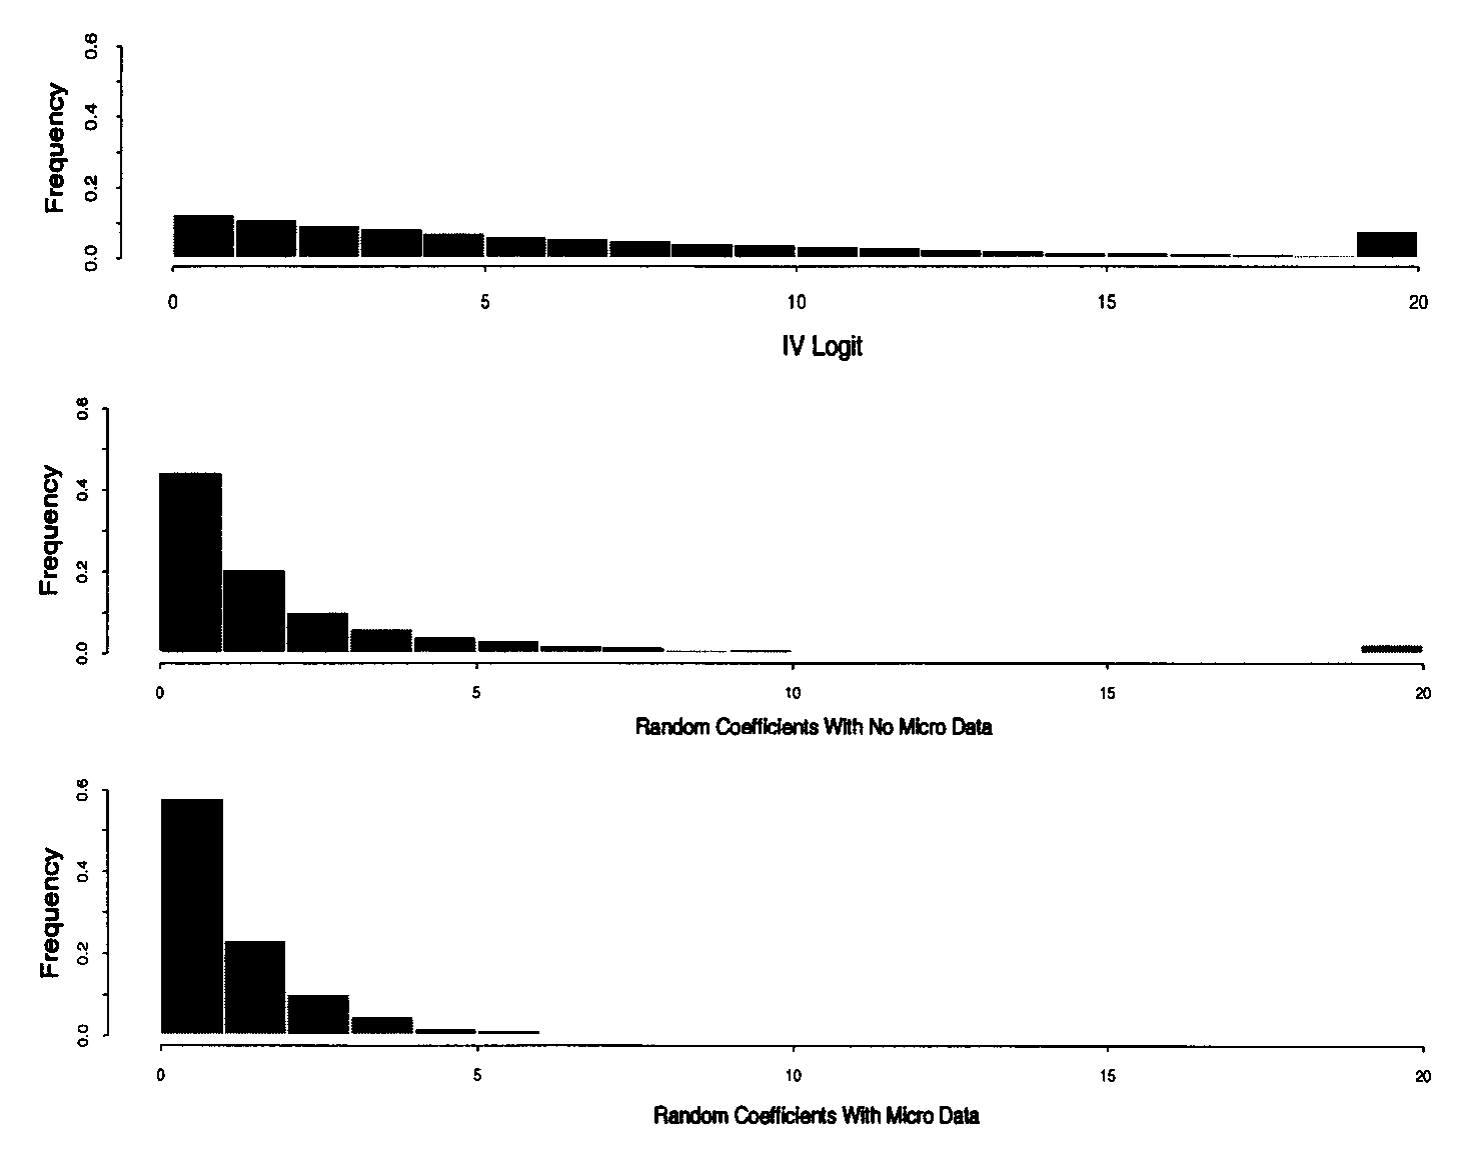
\includegraphics[width=\textwidth]{figures/ch10/petrin_fig1.png}
\caption{Distribution of compensating variation for 1984 minivan buyers, in thousands of 1982--84 dollars. The top
panel is the IV logit model, the middle panel the random coefficients model without micro data, and the bottom panel
the random coefficients model with micro data. The bar at 20 appears to collect the upper tail. Source: Petrin (2002), Figure~1.}
\label{fig:10-petrin-cv-hist}
\end{figure}

\Cref{fig:10-petrin-cv-hist} shows the whole distribution of compensation. Under the IV logit, 10 percent of
minivan buyers would need at least \$20,000 (p.~723). With random coefficients, the tail is much thinner, but many
buyers would still need thousands of dollars. Adding the micro moments removes most of the ``extreme-tastes'' tail.
Petrin prefers the full model on the cumulative weight of this evidence.

\casehead{Markups} \Cref{tab:10-petrin-markups} reproduces Table~9. The two logit models imply mean markups of \$13,904
and \$7,551. Their ratio is almost exactly the ratio of the price coefficients, as the logit markup formula
$\frac{1}{\alpha(1 - S_f)}$ implies (p.~723, n.~14). The same formula explains the tiny dispersion. The standard
deviation is 1.85 percent of the mean in both logit columns, because firms' shares are small and identical across the
two columns.
A Yugo and a Cadillac then carry nearly the same dollar markup. Marginal cost, which is price minus this markup, is
negative for 73.7 percent (OLS) and 22.6 percent (IV) of vehicles. Petrin notes that many logit own-price elasticities
are below one, which is inconsistent with static profit maximization (p.~723, n.~15). The example shows how a bias in
demand passes into the supply side. The random coefficient models imply only positive marginal costs. Their mean
percentage markups are 40.7 percent without micro data and 16.7 percent with them. Both lie within the range of earlier
estimates, 15 to 40 percent in \citet{BerryLevinsohnPakes1995} and an average of 38 percent in \citet{Goldberg1995}
(p.~725, n.~16).

\begin{table}[htbp]
\centering
\caption{Implied markups under Bertrand-Nash pricing, 1981--93 (2,407 models)}\label{tab:10-petrin-markups}
\small
\begin{tabular}{@{}lrrrrrr@{}}
\toprule
 & OLS logit & IV logit & \multicolumn{2}{c}{Random coefficients} & \multicolumn{2}{c}{RC and micro data} \\
\cmidrule(lr){4-5}\cmidrule(l){6-7}
Statistic & (\$) & (\$) & (\$) & (\%) & (\$) & (\%) \\
\midrule
Median              & 13,834 & 7,513 & 2,593 & 36.7 & 1,439 & 15.0 \\
Mean                & 13,904 & 7,551 & 4,017 & 40.7 & 1,753 & 16.7 \\
10th percentile     & 13,647 & 7,413 & 1,628 & 27.8 & 819   & 11.2 \\
90th percentile     & 14,297 & 7,765 & 8,357 & 62.6 & 2,856 & 24.8 \\
Standard deviation  & 257    & 140   & 4,089 & 14.0 & 1,229 & 6.2 \\
Negative marginal costs (\%) & 73.7 & 22.6 & \multicolumn{2}{c}{0} & \multicolumn{2}{c}{0} \\
\bottomrule
\end{tabular}

\smallskip
\begin{minipage}{0.92\textwidth}
\footnotesize Source: \citet[Table~9]{Petrin2002}, 1982--84 CPI-adjusted dollars. Percentage markups are markups
divided by observed prices. They are not reported for the logit models because estimated marginal costs are negative
for many vehicles.
\end{minipage}
\end{table}

Table~10 of the paper follows sales-weighted percentage markups by segment for 1983--87, using the model with micro
data. Minivans earned the highest markups in every year they were sold (19.19 percent in 1984, 19.43 in 1985, 17.33
in 1986 and 16.31 in 1987). Station wagons earned less than minivans in every year. In four of the five years their
markups also fell below those of the column for all other vehicles. The pairs are 18.27 against 18.85 percent in 1983,
16.81 against 17.12 in 1985, 15.82 against 16.43 in 1986 and 13.86 against 14.79 in 1987. In 1984 wagons were slightly
above that column, at 17.83 against 17.72 percent. Petrin's text says that wagon markups ``consistently fell below the
market average'' (p.~725), which his table does not bear out for 1984.
Petrin attributes the minivan premium partly to its location in a less crowded region of product space. Overall,
markups fell as the number of vehicle choices grew from 157 in 1983 to 198 in 1987 (p.~725).

\casehead{Producer surplus and dissipation} \Cref{tab:10-petrin-profits} combines Tables~11 and 12. Chrysler's variable
profits rose by \$202.5 million, or 14.38 percent, in 1984 relative to a world without minivans. The gain grew to
\$504.1 million (32.50 percent) by 1988. Petrin states that by the end of 1987 Chrysler's minivans had generated almost
\$1.5 billion in profits, against a reported development cost of \$700 million (p.~726).\footnote{The Chrysler column
of Table~11 sums to \$1,008.8 million over 1984--87 and to \$1,512.9 million over 1984--88. The paper does not show how
its \$1.5 billion figure is computed. The development cost was reported in \textit{Time} on March 21, 1983. A
\$400 million retooling cost reported in \textit{Fortune} is a lower bound on development costs (p.~726, n.~17).}
Ford and GM were both hurt. The paper summarizes their losses as 1 to 2 percent of variable profits a year, which for
high-volume GM amounted to more than \$100 million in every year of Table~11. Ford's profit rose in 1986, the year its
Aerostar arrived. The industry as a whole lost
in 1984 and 1985, so ex post the industry would have been willing to pay Chrysler not to introduce the minivan
(p.~727). Once Ford and GM sold minivans, they dissipated \$126 million of Chrysler's profits over 1985--88, the
profit on about 76,000 minivans. Chrysler's minivan was differentiated enough to keep much of its market power.

\begin{table}[htbp]
\centering
\caption{Changes in variable profits due to the minivan, and Chrysler's losses to imitators}\label{tab:10-petrin-profits}
\small
\begin{tabular}{@{}lrrrrrrrrr@{}}
\toprule
 & Industry & \multicolumn{2}{c}{Chrysler} & \multicolumn{2}{c}{Ford} & \multicolumn{2}{c}{GM} &
 \multicolumn{2}{c}{Chrysler, dissipation} \\
\cmidrule(lr){3-4}\cmidrule(lr){5-6}\cmidrule(lr){7-8}\cmidrule(l){9-10}
Year & (\%) & (\$m) & (\%) & (\$m) & (\%) & (\$m) & (\%) & (\$m) & (\%) \\
\midrule
1984 & $-0.21$ & 202.5 & 14.38 & $-31.8$ & $-1.16$ & $-155.8$ & $-1.50$ &          &         \\
1985 & $-0.13$ & 259.1 & 13.99 & $-37.4$ & $-1.29$ & $-171.0$ & $-1.63$ & $-6.06$  & $-0.16$ \\
1986 & 0.14    & 201.1 & 12.42 & 54.7    & 1.84    & $-119.9$ & $-1.09$ & $-22.72$ & $-1.99$ \\
1987 & 0.17    & 346.1 & 23.27 & $-22.8$ & $-0.66$ & $-174.5$ & $-2.14$ & $-42.35$ & $-2.25$ \\
1988 & 0.65    & 504.1 & 32.50 & $-24.7$ & $-0.70$ & $-235.4$ & $-2.90$ & $-55.68$ & $-2.63$ \\
\bottomrule
\end{tabular}

\smallskip
\begin{minipage}{0.95\textwidth}
\footnotesize Source: \citet[Tables~11 and 12]{Petrin2002}, model with micro data, millions of 1982--84 dollars. The
first eight columns compare profits with minivans to profits with all minivans removed. The last two compare
Chrysler's profits with all minivans to its profits with the Ford and GM minivans removed.
\end{minipage}
\end{table}

\casehead{Total welfare} \Cref{tab:10-petrin-welfare} reproduces Table~13. Over 1984--88 the compensating variation
sums to \$2,804.55 million and producer profits rise by \$105.54 million, for a welfare gain of \$2,910.09 million.
Producer profits fell in 1984 and 1985 and rose afterward. In every row the welfare change equals the compensating
variation plus the change in producer profits. The gains to society far exceed both the cost of developing the vehicle
and the innovator's private return (p.~727).

\begin{table}[htbp]
\centering
\caption{Change in U.S. welfare from the minivan, 1984--88 (millions of 1982--84 dollars)}\label{tab:10-petrin-welfare}
\small
\begin{tabular}{@{}lrrr@{}}
\toprule
Year & Compensating variation & Change in producer profits & Welfare change \\
\midrule
1984  & 367.29   & $-36.68$ & 330.61 \\
1985  & 625.04   & $-25.07$ & 599.97 \\
1986  & 439.93   & 27.30    & 467.23 \\
1987  & 596.59   & 29.75    & 626.34 \\
1988  & 775.70   & 110.24   & 885.94 \\
\midrule
Total & 2,804.55 & 105.54   & 2,910.09 \\
\bottomrule
\end{tabular}

\smallskip
\begin{minipage}{0.8\textwidth}
\footnotesize Source: \citet[Table~13]{Petrin2002}, model with micro data. Producer profits are the variable profits of
all firms, from the equilibrium with and without minivans.
\end{minipage}
\end{table}

The 1984 numbers can be cross-checked against Table~8. Minivans took 1.58 percent of 10.66 million vehicle sales in
1984, or about 168,000 vehicles (Table~3). Minivan buyers received \$367.29 million less the \$157 million that went to
other households. That leaves about \$1,250 per minivan buyer, close to the mean of \$1,247 in Table~8.

\subsection{Robustness*}\label{sec:10-petrin-robustness}

The paper's main robustness check is the comparison across its four demand models, and we gather its results here.
Instrumenting almost doubles the logit price coefficient (p.~719). Wald tests reject both logit models in favor of
the random coefficients models (p.~719). Without micro data only 6 of the 24 demand parameters have $z$-statistics
above one, and with them 21 of the 24 do (p.~719). Across the four models the mean compensation of 1984 minivan
buyers falls from \$13,652 to \$7,414, \$3,171 and \$1,247 (\cref{tab:10-petrin-cv}). Two further checks discriminate
among the models. The logit models imply negative marginal costs for many vehicles (\cref{tab:10-petrin-markups}).
The random coefficients model without micro data predicts a mean income of minivan buyers far above the CEX value,
while the full model comes close (\cref{tab:10-petrin-cv}). The paper reports no estimates under other taste
distributions. The tail of compensation in \cref{fig:10-petrin-cv-hist} therefore rests on the truncated
$\chi^2(3)$ assumption, which \cref{sec:10-petrin-critique} discusses.

\subsection{Interpretation, limitations and critiques}\label{sec:10-petrin-critique}

The paper's central lesson concerns the logit error. Its share in the welfare of minivan buyers is a diagnostic of how
much the answer rests on the functional form. That share falls from about 700 percent of the mean (the observed part
being negative) under the OLS logit to 32 percent with micro data (\$396 of \$1,247). Even the preferred model credits a
third of the buyers' gain to the $\epsilon_{ij}$ draws. A pure characteristics model would remove that component
entirely \citep{BerryPakes2007}, and \cref{sec:10-charspace} showed that such models value close substitutes much less.
\citet{AckerbergRysman2005} propose a related correction that lets the variance of the logit error shrink as the
product space fills.

Several assumptions shape the level of the estimates. The income term $\alpha_i\ln(y_i - p_j)$ fixes how compensation
scales with income, and the truncated $\chi^2(3)$ distribution fixes the tails of taste heterogeneity. Since compensation
is a nonlinear function of tastes, \cref{fig:10-petrin-cv-hist} depends on these tails. The market size is the number of
U.S. households, so the outside option absorbs all households that buy no new vehicle. The counterfactual holds the
characteristics and the $\xi_j$ of the other vehicles fixed. Ford and GM might have repositioned their wagons or
introduced their own minivans earlier in a world in which Chrysler did not. The model is static, so welfare covers
only 1984--88 and is not discounted. Prices are list prices of base models, without rebates or options.

The counterfactual also defines the object being valued. It removes all minivans, including the Ford and GM models,
so the \$2.9 billion values the minivan as a class of vehicle. The value of any single firm's minivan is a narrower
question. The dissipation counterfactual of Table~12 answers it for the imitators.

Finally, the minivan dummy carries much of the new good's value. A minivan is a new combination of height, size and
front-wheel drive. Its mean taste and the dispersion of that taste ($\pi_{\mathrm{mv}}$) are identified from minivan
sales and from the CEX buyer averages. They are not predicted from tastes for existing characteristics. The
analysis is therefore an ex post valuation, which differs from the ex ante prediction that characteristics models
promise in \cref{sec:10-charspace}.

\subsection{Contribution}\label{sec:10-petrin-contribution}

The paper made two contributions. The first is the micro-moment technique. It brings aggregate information
about buyers into the BLP estimator at almost no computational cost, and it showed that such moments sharpen exactly
the parameters that matter for welfare. Micro moments are now routine in demand estimation (\cref{sec:08-micro}). The
second is the welfare accounting of a new good under oligopoly. Petrin measured how much of the consumer gain came
through competition (43 percent in 1984), how much the innovator earned, and how much the imitators dissipated. He
concludes that large improvements in consumers' standard of living arise from competition among firms that seek
temporary market power through new goods (p.~728).

\begin{table}[htbp]
\centering
\caption{Identification and counterfactual map of Petrin (2002)}
\label{tab:10-petrin-map}
\footnotesize
\renewcommand{\arraystretch}{1.1}
\begin{tabularx}{\textwidth}{@{}>{\raggedright\arraybackslash}p{2.6cm}>{\raggedright\arraybackslash}X@{}}
\toprule
Observed data & Prices, sales and characteristics of 2,407 U.S. nameplate-years, 1981--1993. CEX
  averages of the demographics of new-vehicle buyers, 1987--1992, and the CPS income distribution. \\
\addlinespace
Latent objects & Product quality $\xi_j$, cost shocks $\omega_j$, household tastes and incomes, and
  marginal costs. \\
\addlinespace
Estimated parameters & Price coefficients for three income groups, random-coefficient scales $\sigma_k$,
  family-vehicle interactions $\pi$, mean tastes and the cost coefficients $\gamma$. \\
\addlinespace
Identifying variation & Characteristics-based instruments for prices, as in BLP, plus micro moments that
  match purchase probabilities by income group and the family size and age of the buyers of each vehicle
  type. \\
\addlinespace
Maintained assumptions & Static multiproduct Bertrand-Nash pricing, log-linear marginal cost, the income
  term $\alpha_i\ln(y_i-p_j)$, exogenous characteristics, and a market size equal to the number of
  households. \\
\addlinespace
Counterfactual and what it holds fixed & Removal of all minivans, with the prices of the other vehicles
  re-solved. Marginal costs, characteristics and $\xi_j$ are held fixed. A second counterfactual removes
  only the Ford and GM minivans. \\
\addlinespace
Conclusion & The compensating variation is \$2,804.55 million over 1984--1988, and about 43 percent of the
  consumer gain in 1984 came through lower prices of other vehicles. Micro moments shrink the share of the
  logit errors in buyers' gains. \\
\addlinespace
One limitation & Rivals cannot reposition their products in the counterfactual, although they might have
  done so in a world without Chrysler's minivan. \\
\addlinespace
Source and our additions & The tables are Petrin's. \Cref{prop:10-logit-buyer-cv,lem:10-micro-moment} and the
  diversion form \eqref{eq:10-petrin-diversion} are ours. \\
\addlinespace
Tools in the appendices & \Cref{sec:A-gmm,sec:A-simulation,sec:B-fixedpoint}. \\
\bottomrule
\end{tabularx}
\end{table}

\section{Case study: complementarity and online news (Gentzkow 2007)}\label{sec:10-gentzkow}

Every discrete choice model of this chapter so far assumes that a consumer chooses one product. In those models the
new good can only draw consumers away from existing goods. The continuous demand systems of the chapter, such as the
AIDS system of \cref{sec:10-hausman}, are different, since they let spending spread over many brands.
\citet{Gentzkow2007} builds a discrete choice model in which consumers may choose
several goods at once, and in which the data decide whether goods are substitutes or complements. He applies it to the
\textit{Washington Post}, its online edition (the post.com) and the competing daily \textit{Washington Times}. We follow
the paper from its question to its contribution, and \cref{tab:10-gentzkow-map} at the end of the section maps
it.\footnote{Gentzkow writes $\sigma$ for the correlation of the
unobservables in his two-good model and $\Gamma$ for the interaction term. He writes $\gamma$ for the probability of a
news-day shock, $\lambda$ for the number of readers per copy, $\kappa$ for the transaction cost of online payment and
$\Psi$ for the fixed cost. We write $\rho$, $\Gamma_{AB}$ (or $\Gamma_r$ for bundle $r$), $\varpi$, $\kappa$, $\chi$ and
$F^{\mathrm{fix}}$. Page and table numbers in this section refer to the journal article.}

\subsection{The question}\label{sec:10-gentzkow-question}

Do new goods crowd out existing goods or complement them? Gentzkow opens with examples in which the answer surprised
the industry (p.~713). Record companies in the 1920s believed that radio broadcasts crowded out record sales, until
radio airplay turned out to raise them. A widely cited forecast predicted that computers would create a ``paperless
office,'' yet information technology sharply increased paper consumption. Newspaper executives in the early 2000s
debated whether free online editions siphon readers from print (p.~714, n.~4).

The answer matters for three reasons (pp.~713--714). It drives firms' decisions on entry, positioning and pricing.
It determines the welfare value of the new good and hence the bias of price indexes. It informs policy, such as rules
on cross-media mergers. Standard discrete choice models cannot answer the question. They assume that each consumer
chooses exactly one product, so all goods are perfect substitutes at the individual level (p.~714). The single-unit
assumption is reasonable for cars, and it is the main limitation of characteristics models for goods consumed together.
Gentzkow's model removes it.

A second difficulty is empirical. Frequent online readers are also frequent print readers. The pattern could mean that
the goods are complements. It could also mean that some consumers simply have a stronger taste for news. Separating
true complementarity from correlated tastes is the central identification problem of the paper (p.~714).

\subsection{A two-good model of bundles}\label{sec:10-gentzkow-model}

Consider two goods, $A$ and $B$. Each consumer buys at most one unit of each, so she chooses one of four
\emph{bundles}: nothing ($0$), $A$ only, $B$ only, or both ($AB$). Income not spent on the goods buys a composite good
whose utility is $\alpha$ per dollar. Let $u_r$ be the utility of bundle $r$ relative to the empty bundle. Gentzkow
specifies (p.~717, eq.~1)
\begin{equation}\label{eq:10-gentzkow-twogood}
  u_0 = 0, \qquad u_A = \delta_A - \alpha p_A + \nu_A, \qquad u_B = \delta_B - \alpha p_B + \nu_B, \qquad
  u_{AB} = u_A + u_B + \Gamma_{AB} .
\end{equation}
Here $\delta_A$ and $\delta_B$ are mean utilities, and $(\nu_A, \nu_B)$ are unobserved tastes. The parameters
$\delta_A$, $\delta_B$ and $\Gamma_{AB}$ are common to all consumers. The term $-\alpha p_j$ is the utility of the
composite good forgone, $\alpha(y - p_j) - \alpha y$. The \emph{interaction term}
\begin{equation*}
  \Gamma_{AB} = (u_{AB} - u_B) - (u_A - u_0)
\end{equation*}
is the discrete analog of a cross-partial derivative of utility. It measures how much the added utility of $A$ rises
when $B$ is consumed as well. Gentzkow assumes that $(\nu_A, \nu_B)$ is bivariate normal with unit variances and
correlation $\rho$. One unit variance is a normalization of scale. The other only simplifies exposition.

Demand per consumer is $Q_A = P_A + P_{AB}$ for good $A$ and $Q_B = P_B + P_{AB}$ for good $B$, where $P_r$ is the
probability of choosing bundle $r$. Because utility is quasi-linear, income effects are absent, and compensated and
uncompensated cross-price derivatives coincide. The standard definition of complements \citep{Samuelson1974} then reads
as follows (p.~717, Definition~1).

\begin{definition}[Substitutes and complements]\label{def:10-gentzkow-complements}
Goods $A$ and $B$ are \emph{substitutes} if $\frac{\partial Q_A}{\partial p_B} > 0$, \emph{independent} if
$\frac{\partial Q_A}{\partial p_B} = 0$, and \emph{complements} if $\frac{\partial Q_A}{\partial p_B} < 0$.
\end{definition}

\casehead{Choice regions} The consumer picks the bundle with the highest utility. Comparing the four utilities pairwise
gives the regions of the $(u_A, u_B)$ plane shown in \cref{fig:10-gentzkow-regions}. Bundle $AB$ beats $A$ when $u_B +
\Gamma_{AB} \ge 0$, beats $B$ when $u_A + \Gamma_{AB} \ge 0$, and beats $0$ when $u_A + u_B + \Gamma_{AB} \ge 0$.
Bundle $A$ beats $0$ when $u_A \ge 0$ and beats $B$ when $u_A \ge u_B$. Three cases follow.

If $\Gamma_{AB} = 0$, the comparisons separate. The consumer buys $A$ if and only if $u_A \ge 0$, and $B$ if and only if
$u_B \ge 0$. The boundaries are the two axes.

If $\Gamma_{AB} > 0$, the consumer buys $AB$ when $u_A \ge -\Gamma_{AB}$, $u_B \ge -\Gamma_{AB}$ and $u_A + u_B \ge
-\Gamma_{AB}$. She buys $A$ alone when $u_A \ge 0$ and $u_B \le -\Gamma_{AB}$, and $B$ alone in the mirror case. She buys
nothing when $u_A \le 0$, $u_B \le 0$ and $u_A + u_B \le -\Gamma_{AB}$. The boundary between $AB$ and $0$ is the
segment of the anti-diagonal line $u_A + u_B = -\Gamma_{AB}$ with both coordinates in $[-\Gamma_{AB}, 0]$. Consumers on
that segment are indifferent between buying both goods and buying neither.

If $\Gamma_{AB} < 0$, the consumer buys $AB$ when $u_A \ge -\Gamma_{AB}$ and $u_B \ge -\Gamma_{AB}$. She buys $A$ alone
when $u_A \ge 0$, $u_A \ge u_B$ and $u_B \le -\Gamma_{AB}$, and $B$ alone in the mirror case. She buys nothing when both
utilities are negative. The boundary between $A$ alone and $B$ alone is the segment of the diagonal $u_A = u_B$ with
both coordinates in $[0, -\Gamma_{AB}]$. Consumers on it are indifferent between the two goods.

\begin{figure}[htbp]
\centering
\begin{subfigure}[b]{0.32\textwidth}
\centering
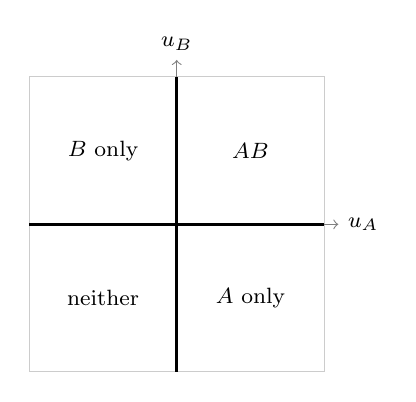
\begin{tikzpicture}[scale=0.72, font=\footnotesize]
  \draw[gray!40] (-2.6,-2.6) rectangle (2.6,2.6);
  \draw[->, gray] (-2.6,0) -- (2.85,0) node[right, black] {$u_A$};
  \draw[->, gray] (0,-2.6) -- (0,2.9) node[above, black] {$u_B$};
  \draw[very thick] (-2.6,0) -- (2.6,0);
  \draw[very thick] (0,-2.6) -- (0,2.6);
  \node at (1.3,1.3) {$AB$};
  \node at (1.3,-1.3) {$A$ only};
  \node at (-1.3,1.3) {$B$ only};
  \node at (-1.3,-1.3) {neither};
\end{tikzpicture}
\caption{$\Gamma_{AB} = 0$}
\end{subfigure}\hfill
\begin{subfigure}[b]{0.32\textwidth}
\centering
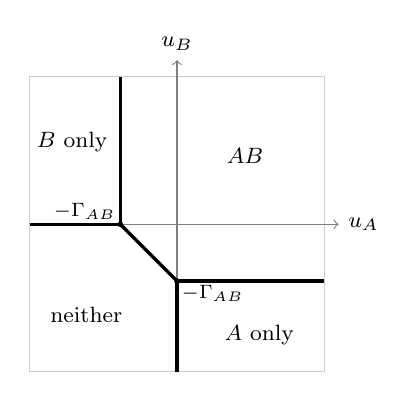
\begin{tikzpicture}[scale=0.72, font=\footnotesize]
  \draw[gray!40] (-2.6,-2.6) rectangle (2.6,2.6);
  \draw[->, gray] (-2.6,0) -- (2.85,0) node[right, black] {$u_A$};
  \draw[->, gray] (0,-2.6) -- (0,2.9) node[above, black] {$u_B$};
  \draw[very thick] (-2.6,0) -- (-1,0) -- (-1,2.6);
  \draw[very thick] (-1,0) -- (0,-1);
  \draw[very thick] (0,-2.6) -- (0,-1) -- (2.6,-1);
  \fill (-1,0) circle (1.4pt);
  \fill (0,-1) circle (1.4pt);
  \node[anchor=south east, inner sep=1.5pt] at (-1,0) {\scriptsize $-\Gamma_{AB}$};
  \node[anchor=north west, inner sep=1.5pt] at (0,-1) {\scriptsize $-\Gamma_{AB}$};
  \node at (1.2,1.2) {$AB$};
  \node at (1.45,-1.95) {$A$ only};
  \node at (-1.85,1.45) {$B$ only};
  \node at (-1.6,-1.6) {neither};
\end{tikzpicture}
\caption{$\Gamma_{AB} > 0$ (complements)}
\end{subfigure}\hfill
\begin{subfigure}[b]{0.32\textwidth}
\centering
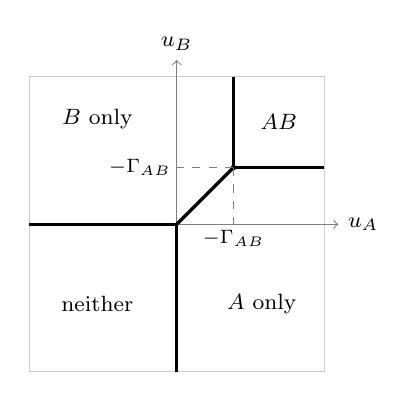
\begin{tikzpicture}[scale=0.72, font=\footnotesize]
  \draw[gray!40] (-2.6,-2.6) rectangle (2.6,2.6);
  \draw[->, gray] (-2.6,0) -- (2.85,0) node[right, black] {$u_A$};
  \draw[->, gray] (0,-2.6) -- (0,2.9) node[above, black] {$u_B$};
  \draw[very thick] (-2.6,0) -- (0,0) -- (0,-2.6);
  \draw[very thick] (0,0) -- (1,1);
  \draw[very thick] (1,2.6) -- (1,1) -- (2.6,1);
  \fill (1,1) circle (1.4pt);
  \draw[gray, dashed] (1,1) -- (1,0);
  \draw[gray, dashed] (1,1) -- (0,1);
  \node[anchor=north, inner sep=2pt] at (1,0) {\scriptsize $-\Gamma_{AB}$};
  \node[anchor=east, inner sep=2pt] at (0,1) {\scriptsize $-\Gamma_{AB}$};
  \node at (1.8,1.8) {$AB$};
  \node at (1.5,-1.4) {$A$ only};
  \node at (-1.4,1.85) {$B$ only};
  \node at (-1.4,-1.4) {neither};
\end{tikzpicture}
\caption{$\Gamma_{AB} < 0$ (substitutes)}
\end{subfigure}
\caption{Choice regions of the two-good bundle model in the plane of $(u_A, u_B)$, the utilities of $A$ and $B$ relative
to buying nothing. Thick lines are indifference boundaries. In panel (b) the anti-diagonal segment $u_A + u_B =
-\Gamma_{AB}$ separates buying both goods from buying neither. In panel (c) the diagonal segment $u_A = u_B$ separates
buying $A$ alone from buying $B$ alone. A rise in $p_B$ shifts probability mass downward. Only consumers on the
diagonal segments change their consumption of $A$. Drawn from the boundaries derived in the text. Compare
\citet[Figure~1]{Gentzkow2007}.}
\label{fig:10-gentzkow-regions}
\end{figure}

\casehead{Why the interaction term decides} A rise in $p_B$ lowers $u_B$ for every consumer and moves probability
mass down in \cref{fig:10-gentzkow-regions}. In panel (a), consumers who move from $AB$ to $A$ alone and from $B$
alone to nothing leave the demand for $A$ unchanged. In panel (b), some consumers on the anti-diagonal segment move
from $AB$ to nothing, so they stop buying $A$. In panel (c), consumers on the diagonal segment move from $B$ alone to
$A$ alone, so they start buying $A$ (pp.~718--719). The following result makes the argument exact.

\begin{proposition}[The interaction term signs the cross-price effect]\label{prop:10-gentzkow-subst}
In the model of \eqref{eq:10-gentzkow-twogood}, let $\alpha > 0$ and let $(\nu_A,\nu_B)$ have a continuous joint density that
is positive on $\R^2$. Write $f_u$ for the implied density of $(u_A, u_B)$. Then
\begin{equation}\label{eq:10-gentzkow-crossderiv}
  \frac{\partial Q_A}{\partial p_B} =
  \begin{cases}
    \alpha\displaystyle\int_0^{-\Gamma_{AB}} f_u(t,t)\,\dd t > 0 & \text{if } \Gamma_{AB} < 0,\\[2ex]
    0 & \text{if } \Gamma_{AB} = 0,\\[1ex]
    -\alpha\displaystyle\int_{-\Gamma_{AB}}^{0} f_u(-\Gamma_{AB} - t,\, t)\,\dd t < 0 & \text{if } \Gamma_{AB} > 0 .
  \end{cases}
\end{equation}
Hence $A$ and $B$ are substitutes if $\Gamma_{AB} < 0$, independent if $\Gamma_{AB} = 0$ and complements if
$\Gamma_{AB} > 0$ \citep[Proposition~1]{Gentzkow2007}.
\end{proposition}

\begin{proof}
\textit{Step 1: the condition for consuming $A$.} Ties have probability zero. The consumer consumes $A$ when her best
bundle containing $A$ beats her best bundle without it:
\begin{align*}
  \max\{u_A,\; u_A + u_B + \Gamma_{AB}\} &\ge \max\{0,\; u_B\}, \\
  u_A + \max\{0,\; u_B + \Gamma_{AB}\} &\ge \max\{0,\; u_B\}, \\
  u_A &\ge g(u_B), \qquad g(b) \equiv \max\{0, b\} - \max\{0, b + \Gamma_{AB}\} .
\end{align*}

\textit{Step 2: the shape of $g$.} If $\Gamma_{AB} = 0$, then $g \equiv 0$. If $\Gamma_{AB} > 0$, then $g(b) = 0$ for $b
\le -\Gamma_{AB}$, $g(b) = -\Gamma_{AB} - b$ for $-\Gamma_{AB} < b < 0$, and $g(b) = -\Gamma_{AB}$ for $b \ge 0$. So $g$ is
nonincreasing with slope $-1$ on $(-\Gamma_{AB}, 0)$. If $\Gamma_{AB} < 0$, then $g(b) = 0$ for $b \le 0$, $g(b) = b$ for
$0 < b < -\Gamma_{AB}$, and $g(b) = -\Gamma_{AB}$ for $b \ge -\Gamma_{AB}$. So $g$ is nondecreasing with slope $+1$ on
$(0, -\Gamma_{AB})$. Outside these intervals $g' = 0$.

\textit{Step 3: differentiate demand.} Write $c_A = \delta_A - \alpha p_A$ and $c_B = \delta_B - \alpha p_B$, so that
$u_A = c_A + \nu_A$ and $u_B = c_B + \nu_B$. Let $f$ be the density of $(\nu_A, \nu_B)$. Then
\begin{equation*}
  Q_A = \Pr\bigl(\nu_A \ge g(c_B + \nu_B) - c_A\bigr)
      = \int_{-\infty}^{\infty}\int_{g(c_B + \nu_B) - c_A}^{\infty} f(\nu_A, \nu_B)\,\dd\nu_A\,\dd\nu_B .
\end{equation*}
The function $g$ is piecewise linear, so we may differentiate under the outer integral:
\begin{align*}
  \frac{\partial Q_A}{\partial c_B} &= -\int_{-\infty}^{\infty} f\bigl(g(c_B + \nu_B) - c_A,\, \nu_B\bigr)\,
         g'(c_B + \nu_B)\,\dd\nu_B
      = -\int_{-\infty}^{\infty} f_u\bigl(g(t),\, t\bigr)\, g'(t)\,\dd t ,
\end{align*}
where the second equality substitutes $t = c_B + \nu_B$ and uses $f_u(a,b) = f(a - c_A, b - c_B)$. Since $\frac{\partial
c_B}{\partial p_B} = -\alpha$,
\begin{equation*}
  \frac{\partial Q_A}{\partial p_B} = \alpha\int_{-\infty}^{\infty} f_u\bigl(g(t),\, t\bigr)\, g'(t)\,\dd t .
\end{equation*}

\textit{Step 4: evaluate.} If $\Gamma_{AB} = 0$, then $g' \equiv 0$ and the derivative is zero. If $\Gamma_{AB} < 0$, then
$g(t) = t$ and $g'(t) = 1$ on $(0, -\Gamma_{AB})$, which gives the first line of \eqref{eq:10-gentzkow-crossderiv}. If
$\Gamma_{AB} > 0$, then $g(t) = -\Gamma_{AB} - t$ and $g'(t) = -1$ on $(-\Gamma_{AB}, 0)$, which gives the third line.
The density is positive, so both integrals are strictly positive.
\end{proof}

The two integrals run along the diagonal segments of \cref{fig:10-gentzkow-regions}. Gentzkow's equation~(3) writes
them as line integrals with indicator functions (p.~719). The magnitude of the cross effect depends on the length
$|\Gamma_{AB}|$ of the segment and on the density of consumers along it. The proposition also covers nonprice shifters.
Suppose a variable $z$ raises $u_B$ by $\zeta z$ and leaves $u_A$ unchanged. Then $\frac{\partial Q_A}{\partial z} =
\zeta\frac{\partial Q_A}{\partial c_B} = -\frac{\zeta}{\alpha}\frac{\partial Q_A}{\partial p_B}$. Improving the
connection speed of an online paper works like cutting its price, and its effect on print demand has the sign of
$\Gamma_{AB}$ (p.~719). This is how Gentzkow's excluded variables reveal substitution without any price variation.

\subsection{What the data can and cannot identify}\label{sec:10-gentzkow-ident}

\casehead{A counting problem} Choice data in the two-good model give three probabilities, $P_A$, $P_B$ and $P_{AB}$.
The model has five parameters: $\delta_A$, $\delta_B$, $\Gamma_{AB}$, $\rho$ and $\alpha$ (p.~720). The price
coefficient is identified from choices only if prices vary, because the probabilities depend on $(\delta_A, \delta_B,
\alpha)$ only through $\delta_A - \alpha p_A$ and $\delta_B - \alpha p_B$. Without price variation, $\alpha$ needs
another moment. Gentzkow takes it from a firm's pricing condition (\cref{sec:10-gentzkow-supply}).

The harder problem is to separate $\Gamma_{AB}$ from $\rho$. The marginal probabilities $Q_A$ and $Q_B$ identify the two
mean utilities. One moment remains, how often the goods are consumed together. A high $P_{AB}$ relative to $P_A$ and
$P_B$ can come from a large $\Gamma_{AB}$ or from a large $\rho$, and nothing else in the data separates them
(p.~720). By \cref{prop:10-gentzkow-subst}, the same data could be fit by near-perfect substitutes with highly
correlated tastes, or by near-perfect complements with weakly correlated tastes. A model that fixes one of the two
parameters by assumption fixes the answer to the substitution question.

\casehead{Exclusion restrictions} Suppose a variable $x$ enters the utility of $A$ only. Observing choices at a second
value of $x$ adds three moments, $P_A$, $P_B$ and $P_{AB}$ at the new value, and one parameter, the new mean utility of
$A$ (p.~721). The model becomes formally identified. The intuition is direct. If joint consumption reflects a high
$\Gamma_{AB}$, then shifting up the utility of $A$ raises the probability of consuming $B$. If it reflects correlated
tastes, the probability of consuming $B$ stays unchanged. \citet{Keane1992} gives Monte Carlo evidence that exclusion
restrictions sharpen the covariance estimates of multinomial probit models, which nest the model of \eqref{eq:10-gentzkow-twogood}
when defined over bundles (p.~721, n.~11).

\casehead{Panel data} Split each taste into a consumer random effect, constant over time, and a shock that is \iid\
across goods and days. With choices observed at two dates there are $4^2 = 16$ joint outcomes, hence 15 moments
instead of 3 (p.~721, n.~12). The argument is the usual one for random effects. Correlated random effects make some
consumers likely to consume both goods and others likely to consume neither. Conditional on a consumer's average
propensities, her day-to-day variation is then uncorrelated across goods. A high $\Gamma_{AB}$ instead makes the
day-to-day variation strongly correlated. The consumer reads both papers on some days and neither on others, and
rarely reads only one.

Gentzkow's data are a limited panel. Respondents report what they read in the last 24 hours and in the last five
weekdays. For consumers who read nothing in the last 24 hours, the five-day report shows which papers they read on
the other four weekdays. Whether they
were less likely to read then identifies the variance of the random effects. Consumers who read one paper in the last
24 hours identify the correlation. If the random effects are positively correlated, a consumer who read only $A$
yesterday is more likely to have read $B$ earlier in the week (p.~722).

\casehead{Unobserved goods} The outside option has a different meaning when bundles are allowed. Every choice in the
model includes an implicit maximization over goods the econometrician does not see, such as cable news (p.~719).
Suppose watching CNN destroys the value of the post.com and raises the value of the print \textit{Post}. Then the
\textit{Post} and the post.com are never read together, and the model estimates them as strong substitutes. Gentzkow
argues that this answer is correct for the market as it is. Raising the price of the \textit{Post} would reduce CNN
viewing as well and raise post.com reading (p.~720). The estimates are conditional on the set and the prices of the
unobserved goods, a limitation all discrete choice models share \citep{Samuelson1974}.

\casehead{Relation to earlier models} The model of \eqref{eq:10-gentzkow-twogood} nests the earlier approaches as restrictions
(pp.~722--723). The multiple-discrete choice model of \citet{Hendel1999} aggregates many ``tasks,'' such as the
computing needs of each employee of a firm. Hendel's model lets a buyer choose several units of several brands, and he
estimates it by the method of simulated moments on micro data for personal computer purchases by firms. Each task uses
one good, so the task-level model fixes $\Gamma_{AB} = -\infty$, and the goods are restricted to be substitutes
(\cref{ch:logit}). A multivariate probit, with one equation per good and correlated errors, sets $\Gamma_{AB} = 0$
and forces independence. A logit or nested logit over bundles \citep{ManskiSherman1980,TrainMcFaddenBenAkiva1987} can
estimate $\Gamma_{AB}$ freely. Its unobservables, however, are uncorrelated or follow the nest structure, so it would
read correlated tastes as complementarity. Gentzkow's model frees both terms and relies on exclusions and panel
information to separate them.

\subsection{Setting and data}\label{sec:10-gentzkow-data}

The data come from a Scarborough Research survey of 16,179 adults in the Washington, DC, Designated Market Area (DMA),
conducted between March 2000 and February 2003 (p.~723). The survey lists the local print newspapers each respondent
read in the last 24 hours and in the last five weekdays. It records the readership of the major local online newspapers
over the same windows, and many household characteristics. The \textit{Post} dominated the market, with an average daily readership
of 1.8 million against 256,000 for the \textit{Times}. The post.com had 406,000 area readers per day. The
\textit{Times}'s own website had only 373 readers in the sample and is omitted (p.~723, n.~16). The goods are the daily
editions of the \textit{Post}, the \textit{Times} and the post.com. The outside option includes all other news
sources and not reading news at all.

The survey is about a 0.4 percent sample and broadly representative. It overrepresents older, more educated and
wealthier residents and underrepresents minorities (p.~724). Estimation uses the unweighted data, and the policy
simulations use the sampling weights. About 6 percent of records were filled in by Scarborough from matched
respondents. Gentzkow drops them in estimation and keeps them in the simulations (p.~724, n.~17).

The aggregate time series are suggestive but inconclusive (p.~724). Post.com readership grew rapidly after its
introduction in 1996 while \textit{Post} readership fell. A regression of \textit{Post} readership since 1984 on
post.com readership and a trend implies that four post.com readers displace one \textit{Post} reader. Yet the decline
began in 1994, two years before the post.com, and did not accelerate afterward. Readership was falling nationally, and
the \textit{Post} raised its subscription price several times. Time series alone cannot separate these forces.

The micro data show that reading several papers is common (p.~725). Forty-eight percent of respondents read at least
one of the three papers in the last 24 hours. Of these, 18 percent read two and 1 percent read all three. Over five
days, 65 percent read at least one, and of these 27 percent read two and 3 percent all three. Panel~A of
\cref{tab:10-gentzkow-data} cross-tabulates \textit{Post} and post.com readership. Among post.com readers the share who
also read the \textit{Post} is higher than among non-readers. Panel~B reports raw and partial correlations. The partial
correlations control for age, sex, education, occupation, employment status, income, political party, survey date,
location and the number of missing answers. Controls cut the \textit{Post}-post.com correlation by about two-thirds,
but it stays significantly positive. The \textit{Post}-\textit{Times} correlation is positive in the raw data and
vanishes or turns negative with controls.

\begin{table}[htbp]
\centering
\caption{Joint readership of the \textit{Post}, the post.com and the \textit{Times}}\label{tab:10-gentzkow-data}
\small
\begin{tabular}{@{}lrrrr@{}}
\toprule
\multicolumn{5}{@{}l}{\textit{A. Cross-tabulation of Post and post.com readership (number of respondents)}} \\
 & \multicolumn{2}{c}{Last 24 hours} & \multicolumn{2}{c}{Last 5 weekdays} \\
\cmidrule(lr){2-3}\cmidrule(l){4-5}
 & No post.com & Read post.com & No post.com & Read post.com \\
\midrule
Did not read \textit{Post} & 8,771 & 622 & 6,012 & 680 \\
Read \textit{Post}         & 5,829 & 877 & 7,203 & 2,204 \\
\midrule
\multicolumn{5}{@{}l}{\textit{B. Correlation coefficients of readership indicators}} \\
 & \multicolumn{2}{c}{Last 24 hours} & \multicolumn{2}{c}{Last 5 weekdays} \\
\cmidrule(lr){2-3}\cmidrule(l){4-5}
 & Raw & Partial & Raw & Partial \\
\midrule
\textit{Post} and post.com        & 0.0989$^{**}$ & 0.0364$^{**}$ & 0.1579$^{**}$ & 0.0673$^{**}$ \\
\textit{Post} and \textit{Times}  & 0.0632$^{**}$ & 0.0035        & 0.0450$^{**}$ & $-0.0623^{**}$ \\
\textit{Times} and post.com       & 0.0146        & 0.0090        & 0.0184        & 0.0066 \\
\bottomrule
\end{tabular}

\smallskip
\begin{minipage}{0.92\textwidth}
\footnotesize Source: \citet[Tables~2 and 3]{Gentzkow2007}, Scarborough survey, Washington, DC, DMA, 2000--03.
Partial correlations are correlations of the residuals from regressions of each readership indicator on the controls
listed in the text. Panel~B drops respondents for whom print or online papers are not in the choice set.
$^{**}$ significant at 1 percent.
\end{minipage}
\end{table}

\subsection{Reduced-form evidence}\label{sec:10-gentzkow-reduced}

To separate complementarity from correlated tastes, Gentzkow uses four variables that shift the utility of reading
online but not, directly, the utility of reading print (pp.~725--726). They are indicators for Internet access at work,
use of the Internet for work-related tasks, use of the Internet for education-related tasks, and a high-speed
connection at home. Access at work lowers the time cost of reading online. The two use variables indicate familiarity
with the Internet and time spent at a computer. A fast connection raises the utility of online reading. Collect them
in a vector $z_i$. No variable shifts the \textit{Post} without shifting the \textit{Times}, so print-print
substitution is less well identified than print-online substitution (p.~726).

A linear probability model shows the exclusion restrictions at work. Let $R^p_i$ indicate that respondent $i$ read the
\textit{Post} in the last five weekdays and $R^w_i$ that she read the post.com. Gentzkow estimates
\begin{equation}\label{eq:10-gentzkow-lpm}
  R^p_i = b\,R^w_i + x_i\varphi + e_i ,
\end{equation}
first by OLS and then by two-stage least squares (2SLS) with $z_i$ as instruments for $R^w_i$. The controls $x_i$ are
those of the partial correlations, plus \textit{Times} readership. The 2SLS coefficient has a simple interpretation in
terms of \cref{prop:10-gentzkow-subst}. Each instrument moves only the utility of the post.com, so it acts like a change
in the post.com's price. The 2SLS coefficient is the ratio of the instrument's effect on \textit{Post} reading to its
effect on post.com reading. In the language of \cref{ch:diffprod}, it estimates minus the diversion ratio from the
post.com to the \textit{Post}, averaged over the respondents whom the instruments move.

\Cref{tab:10-gentzkow-lpm} reproduces Table~4. OLS gives a positive coefficient, 0.0464 (0.0090), which mirrors the
raw correlation. 2SLS gives $-0.4132$ (0.107). Taken literally, a respondent assigned to read the online paper at zero
time cost would be about 41 percentage points less likely to read the print paper. Gentzkow describes this as
``40 percent less likely'' (p.~726). The coefficient on a binary regressor in a linear probability model is a change
in the probability itself. A relative decline would require dividing by a baseline probability of reading the
print paper. Gentzkow warns that the linear
probability model limits how far this magnitude can be trusted. The first-stage $F$-statistic on the instruments is
33.05, so weak instruments are not a concern. The overidentification statistic is $\chi^2 = 3.65$ with a $p$-value of
0.302, so the test does not reject the validity of the instruments.

\begin{table}[htbp]
\centering
\caption{Linear probability model of \textit{Post} readership in the last five weekdays}\label{tab:10-gentzkow-lpm}
\small
\begin{tabular}{@{}lcccc@{}}
\toprule
 & OLS & \multicolumn{3}{c}{2SLS} \\
\cmidrule(l){3-5}
 &  & (1) & (2) & (3) \\
\midrule
Read post.com last 5 days & 0.0464$^{**}$ & $-0.4132^{**}$ & $-0.4579^{**}$ & $-0.4381^{**}$ \\
                          & (0.0090)      & (0.107)        & (0.119)        & (0.141) \\
Other Internet news       &               &                &                & 0.0244 \\
                          &               &                &                & (0.0195) \\
Industry and occupation controls &        &                & Yes            &  \\
Overidentification $p$-value &            & 0.302          & 0.431          & 0.219 \\
$R^2$                     & 0.333         & 0.214          & 0.207          & 0.202 \\
$N$                       & 14,313        & 14,313         & 14,313         & 14,313 \\
\bottomrule
\end{tabular}

\smallskip
\begin{minipage}{0.92\textwidth}
\footnotesize Source: \citet[Table~4]{Gentzkow2007}. Robust standard errors in parentheses. The instruments are
indicators for Internet access at work, a fast Internet connection, and use of the Internet for research or education
and for work. The overidentification test is a Sargan test. Industry controls are 12 categories and occupation
controls 11. All regressions include the controls listed in the text and omit respondents without print papers in the
choice set. $^{**}$ significant at 1 percent.
\end{minipage}
\end{table}

The main threat is that the instruments correlate with unmeasured tastes for print (pp.~727--728). People who like
reading may select into jobs with Internet access, and news enthusiasts may buy fast connections. Gentzkow offers three
checks. Adding 12 industry and 11 occupation categories, which should absorb part of any omitted job characteristic,
strengthens the 2SLS coefficient slightly to $-0.4579$ \citep{AltonjiElderTaber2005}. Restricting the sample to
residents of more than ten years, whose job choices largely predate online news, leaves the estimates nearly unchanged
(p.~727, n.~19). Controlling for other Internet news use raises the coefficient's magnitude slightly ($-0.4381$), so the
instruments do not appear to work through other online news sources. The structural robustness checks below also drop
the broadband exclusion.

\subsection{The empirical model}\label{sec:10-gentzkow-structural}

Index days by $t$, consumers by $i$, goods by $j \in \{1, \dots, J\}$ with $J = 3$, and bundles by $r \in \{0, 1, \dots,
2^J - 1\}$, where $r = 0$ is the empty bundle (p.~728). The utility of consumer $i$ from good $j$ alone on day $t$ is
\begin{equation}\label{eq:10-gentzkow-base}
  \tilde u_{ijt} = \delta_j - \alpha p_j + x_i\beta_j + \nu_{ij} + \tau_{it} .
\end{equation}
The vector $x_i$ holds age, sex, education, occupation, employment status, political party, location within the DMA,
the number of missing survey answers, six-month time dummies and log income. For the post.com it also holds the four
excluded variables $z_i$, which are absent from the print utilities. The time dummies absorb changes in the quality of
the goods and their substitutes. Log income proxies for unobservables correlated with income, since the budget effect
of income differences out (p.~729).

The two unobservables play different roles. The vector $\nu_i = (\nu_{i1}, \dots, \nu_{iJ})$ is constant over the
survey week. It captures a general taste for news, loyalty to a paper and subscription status. It is multivariate
normal with a free covariance matrix, whose scale is pinned down by the logit errors below (p.~729, n.~21). The day
shock $\tau_{it}$ raises the utility of all papers equally. It equals $\hat\tau > 0$ with probability $\varpi$ and zero
otherwise, a stylized description of major news days and of day-to-day variation in the cost of time. Price does not
vary enough to estimate $\alpha$ from demand, so the first two terms are combined into $\bar\delta_j = \delta_j - \alpha
p_j$.

The utility of bundle $r$ adds the base utilities of its goods, an interaction term and a bundle-specific shock
(p.~729, eq.~4):
\begin{equation}\label{eq:10-gentzkow-bundle}
  u_{irt} = \begin{cases}
    \epsilon_{irt} & \text{if } r = 0, \\
    \sum_{j \in r}\tilde u_{ijt} + \Gamma_r + \epsilon_{irt} & \text{if } r > 0.
  \end{cases}
\end{equation}
Here $\Gamma_r = 0$ for single-good bundles, and $\epsilon_{irt}$ is \iid\ type-I extreme value. With three goods there
are three pairwise interactions and one triple interaction, which is estimated but not reported (Table~6, note). On a
major news day the bundle $r$ gains $|r|\hat\tau$, where $|r|$ is its number of goods. The interaction terms and the
price coefficient are common to all consumers. Gentzkow reports that letting $\Gamma_r$ vary with observables did not
change the results substantially (p.~729).

\Cref{prop:10-gentzkow-subst} does not apply unchanged to this model. Label the goods $A$, $B$ and $C$. With three
goods, a change in $p_B$ also moves consumers into and out of the bundles that contain $C$. The triple interaction
and the bundle-specific logit errors then enter the cross-price effect, and a negative $\Gamma_{AB}$ no longer
signs it. Our computation gives an example with $\nu_i$ and $\tau_{it}$ set to zero. Let every
$\bar\delta_j + x_i\beta_j$ be zero, $\alpha = 1$, $\Gamma_{AB} = -1$, $\Gamma_{AC} = \Gamma_{BC} = 0$, and
$\Gamma_r = 10$ for the bundle $r$ of all three goods. With $r_i$ the bundle that consumer $i$ chooses, the logit form
gives $\frac{\partial Q_A}{\partial p_B} = -\alpha\Cov\bigl(\indic\{A\in r_i\},\indic\{B\in r_i\}\bigr) \approx -0.00009$.
So $A$ and $B$ are complements although $\Gamma_{AB} < 0$, because almost every consumer buys all three goods. A
small positive variance of $\nu_i$ preserves the sign. In the empirical model the two-good result is therefore an
intuition, and the substitution patterns must be read from the cross-price derivatives of the full model.

Two dummies define choice sets. About 10 percent of respondents say they look at no newspaper sections, and print
papers are removed from their choice set. Respondents who did not use the Internet in the last 30 days have no online
paper. Each dummy also enters, as a control, the utility of the goods it does not exclude (p.~729). Choice-set
variation therefore does not identify substitution, which seems prudent because it is unlikely to be exogenous
(n.~25).

\casehead{Choice probabilities and the likelihood} Integrating over the $\epsilon_{irt}$ gives the logit probability of
bundle $r$ on a day with shock $\tau$:
\begin{equation}\label{eq:10-gentzkow-Q}
  Q_r(x_i, \nu_i, \tau; \theta) = \frac{\exp\Bigl[\sum_{j\in r}(\bar\delta_j + x_i\beta_j + \nu_{ij} + \tau) + \Gamma_r\Bigr]}
  {1 + \sum_{r'=1}^{2^J - 1}\exp\Bigl[\sum_{j\in r'}(\bar\delta_j + x_i\beta_j + \nu_{ij} + \tau) + \Gamma_{r'}\Bigr]} .
\end{equation}
The data report, for each good, whether it was read in the last 24 hours and whether it was read in the last five
weekdays. Let $\tilde q \in \{0, \dots, 2^J - 1\}^5$ list the bundles chosen on the five weekdays. Let $q$ be a reported
outcome and $\Omega(q)$ the set of daily sequences consistent with it. Since $\tau_{it}$ and $\epsilon_{irt}$ are
independent across days, the probability of report $q$ given $\nu_i$ is (p.~730)
\begin{equation}\label{eq:10-gentzkow-Pq}
  P_q(x_i, \nu_i; \theta) = \sum_{\tilde q \in \Omega(q)}\prod_{t=1}^{5}\Bigl[\varpi\,Q_{\tilde q_t}(x_i, \nu_i, \hat\tau;
  \theta) + (1 - \varpi)\,Q_{\tilde q_t}(x_i, \nu_i, 0; \theta)\Bigr] .
\end{equation}
The log-likelihood integrates over the random effects:
\begin{equation}\label{eq:10-gentzkow-loglik}
  L(X, q, \theta) = \sum_i \ln\int P_{q_i}(x_i, \nu; \theta)\,\dd F(\nu; \theta),
\end{equation}
where $F(\nu; \theta)$ is the multivariate normal distribution of $\nu$ (p.~732, eq.~6).

\casehead{Identification in the empirical model} The two-good intuition carries over (p.~730). The combination of
24-hour and 5-day reports pins down the covariance matrix of $\nu_i$. Choices on earlier days are more correlated with
the choice in the last 24 hours, conditional on observables, the larger the variance of the random effects. The
exclusion restrictions then pin down the distribution of the common day shock $\tau_{it}$ and the interaction terms. If
same-day joint reading of print and online papers is driven by $\tau_{it}$, Internet access at work should not change
the probability of reading print. If it is driven by complementarity, those with access should read print more.
Gentzkow stresses three limitations. The partial panel identifies the random effects less well than a true panel.
The excluded variables shift only the online paper. And without price variation, functional forms carry more weight
than in richer data sets.

\subsection{Simulated maximum likelihood}\label{sec:10-gentzkow-sml}

The integral in \eqref{eq:10-gentzkow-loglik} has no closed form. Gentzkow replaces it with a simulator and maximizes
the simulated likelihood (p.~732, eq.~7):
\begin{equation}\label{eq:10-gentzkow-sml}
  \hat\theta^{SML} = \argmax_\theta \sum_i \ln\Bigl[\frac{1}{S}\sum_{s=1}^{S}P_{q_i}(x_i, \nu_{is}; \theta)\Bigr],
\end{equation}
with $S = 300$ draws per consumer. The leading alternative is the method of simulated moments (MSM) of
\citet{McFadden1989} and \citet{PakesPollard1989}. MSM is consistent for a fixed number of draws. Simulated maximum
likelihood (SML), introduced by \citet{LermanManski1981}, needs the number of draws to grow with the sample
\citep{GourierouxMonfort1996}. But efficient MSM requires optimal instruments, which perform poorly when the
preliminary estimate is inaccurate, and it requires the probabilities of all possible reports. With many reported
outcomes this is expensive. In preliminary tests the two estimators gave similar parameters, and MSM took 10 to 20 times
longer, so Gentzkow uses SML (p.~732).

\casehead{Importance sampling} Draws from the unconditional distribution of $\nu$ waste effort on values that make the
observed report unlikely. Gentzkow instead draws from the distribution of $\nu$ conditional on the observed report,
computed at a preliminary estimate $\tilde\theta$ (p.~732, n.~31). The logic is clearest when the draws are standardized
shocks $\eta \sim N(0, I)$ with density $\phi$, and $\nu = C(\theta)\eta$. (In this subsection $\eta$ and $\phi$
denote these shocks and their density, not the CES elasticity of \cref{sec:10-feenstra}.) Write $P_i(\eta; \theta) \equiv
P_{q_i}(x_i, C(\theta)\eta; \theta)$ for the probability of $i$'s report given the shocks. Let $\bar P_i(\tilde\theta) = \int
P_i(\eta; \tilde\theta)\phi(\eta)\,\dd\eta$, computed once with many draws. The importance density is
\begin{equation*}
  h_i(\eta) = \frac{P_i(\eta; \tilde\theta)\,\phi(\eta)}{\bar P_i(\tilde\theta)} ,
\end{equation*}
which is the posterior density of $\eta$ given the report. The weighted simulator
\begin{equation*}
  \tilde P_i(\theta) = \frac{1}{S}\sum_{s=1}^{S}P_i(\eta_s; \theta)\,W_{is}, \qquad
  W_{is} = \frac{\bar P_i(\tilde\theta)}{P_i(\eta_s; \tilde\theta)}, \qquad \eta_s \sim h_i,
\end{equation*}
is unbiased for every $\theta$:
\begin{equation*}
  \E_h\bigl[P_i(\eta; \theta)\,W_i\bigr]
  = \int P_i(\eta; \theta)\,\frac{\bar P_i(\tilde\theta)}{P_i(\eta; \tilde\theta)}\,
    \frac{P_i(\eta; \tilde\theta)\,\phi(\eta)}{\bar P_i(\tilde\theta)}\,\dd\eta
  = \int P_i(\eta; \theta)\,\phi(\eta)\,\dd\eta .
\end{equation*}
Draws from $h_i$ are taken by acceptance and rejection, since $h_i$ is the distribution of the shocks conditional on the
observed report. \emph{Acceptance and rejection} draws $\eta$ from $\phi$ and keeps each draw with probability
proportional to $P_i(\eta;\tilde\theta)$, so the kept draws follow $h_i$. Gentzkow writes the same simulator in terms of $\nu$ (his eqs.~13--14). The general treatment of
importance sampling is in \cref{sec:08-importance}.

\casehead{Bias correction} SML is biased in finite samples because the logarithm is concave (p.~732, n.~32). Let
$\tilde f$ be an unbiased simulator of a choice probability $f$, so $\E\tilde f = f$. A second-order expansion of $\ln
\tilde f$ around $f$ gives
\begin{align*}
  \ln\tilde f &= \ln f + \frac{\tilde f - f}{f} - \frac{(\tilde f - f)^2}{2f^2} + O\bigl(|\tilde f - f|^3\bigr), \\
  \E\ln\tilde f &\approx \ln f - \frac{1}{2}\,\frac{\E(\tilde f - f)^2}{f^2} = \ln f - \frac{1}{2}\,\frac{\Var(\tilde f)}{f^2} .
\end{align*}
The expected simulated log-likelihood is too low by about half the squared coefficient of variation of the simulator.
If $\tilde f = \frac{1}{S}\sum_s P_{is}$ averages $S$ independent draws, then $\Var(\tilde f) = \frac{1}{S}\Var(P_{is})$,
which can be estimated by $\frac{1}{S^2}\sum_s(P_{is} - \tilde f)^2$. The corrected objective adds this estimate back:
\begin{equation}\label{eq:10-gentzkow-biascorr}
  \hat\theta = \argmax_\theta\sum_i\Biggl\{\ln\tilde f_i + \frac{1}{2}\,
  \frac{\frac{1}{S^2}\sum_{s}\bigl(P_{is} - \tilde f_i\bigr)^2}{\tilde f_i^2}\Biggr\} .
\end{equation}
The correction removes the bias of order $\frac{1}{S}$ \citep[p.~45]{GourierouxMonfort1996}.\footnote{The version of
\eqref{eq:10-gentzkow-biascorr} printed in Gentzkow's footnote 32 does not show the factor $\frac{1}{S^2}$ in the
correction term. We state the expression that follows from the expansion.} The robust standard errors follow
\citet{McFaddenTrain2000}. For welfare and other derived statistics, Gentzkow draws 100 parameter vectors from the
estimated asymptotic distribution, recomputes the statistic at each, and reports the standard deviation (p.~733). This
avoids the delta method, which linearizes highly nonlinear functions.

\subsection{The price coefficient from the supply side}\label{sec:10-gentzkow-supply}

Demand data identify only $\bar\delta_j = \delta_j - \alpha p_j$. To express utility in dollars, Gentzkow backs out
$\alpha$ from the condition that the \textit{Post} sets its print price optimally (pp.~730--731 and 735--736). The idea
is that the less price-sensitive consumers are, the higher the price a profit-maximizing firm would set (p.~715).

\casehead{Profit} The \textit{Post} sells copies at price $p$, and each copy is read by $\kappa$ adults. The firm
earns advertising revenue $a_p$ per print reader and $a_w$ per online reader, pays marginal cost $c_p$ per printed copy,
and bears a fixed cost. With $N_p$ print readers and $N_w$ online readers, the profit of the Washington Post Company is
(p.~731, eq.~5)
\begin{equation}\label{eq:10-gentzkow-profit}
  \Pi = \Bigl[a_p + \frac{p - c_p}{\kappa}\Bigr]N_p + a_w N_w - F^{\mathrm{fix}} .
\end{equation}
The marginal cost of an extra online reader is taken to be zero, and advertising revenue per reader is constant. The
second assumption treats both advertising markets as competitive at a fixed price per reader. It abstracts from the
different values of different readers and from any market power of the \textit{Post} (p.~735). Since $\kappa$ readers
share each copy, Gentzkow assumes that each reader pays $\frac{p}{\kappa}$ and that this reader price enters the
utility \eqref{eq:10-gentzkow-base} (p.~731).

\casehead{Inputs} Every input comes from industry data (pp.~735--736).
\begin{itemize}
  \item Print advertising revenue was \$574.3 million in 2001 and \$555.7 million in 2002. The daily edition's share
        gives \$1.5 and \$1.4 million per day, and with daily circulation of 771,614 and 768,600 the average is $a_p =
        \$1.91$.
  \item Online division revenue was \$30.4 million in 2001 and \$35.9 million in 2002. The post.com had 450,457 daily
        readers in the DMA, about 75 percent of its total. Dividing 75 percent of revenue by DMA readership gives
        $a_w = \$0.15$. A second estimate from the advertising revenue and readership of nytimes.com gives \$0.16,
        which Gentzkow uses.
  \item Newsprint consumption of 226,796 metric tons at \$541 per ton implies \$0.37 per copy. With ink and distribution,
        $c_p = \$0.40$.
  \item The cover price rose from \$0.25 to \$0.35 over the period, and the subscription price per daily copy was
        \$0.22 to \$0.25. Gentzkow uses $p = \$0.30$.
  \item Comparing survey readership with audited circulation gives $\kappa = 2.4$ readers per copy (2.3 for the
        \textit{Times}). Whether $\kappa$ reflects shared copies or overreporting does not change the welfare results
        (p.~731, n.~28).
\end{itemize}
The profit from one more print reader is \$0.75, and from one more online reader \$0.16 (p.~736).\footnote{With the
reported inputs, $\frac{a_p + p - c_p}{\kappa} = \frac{1.91 + 0.30 - 0.40}{2.4} = 0.754$, which reproduces the \$0.75
in the paper. The bracket of \eqref{eq:10-gentzkow-profit} as printed, $a_p + \frac{p - c_p}{\kappa}$, would give about
\$1.87. The reported figure is therefore consistent with $a_p$ measured per copy, which is how it is computed from
circulation.}

\casehead{The first-order condition} Write the expected numbers of print and online readers as functions $N_p(\bar
\delta; \hat\theta)$ and $N_w(\bar\delta; \hat\theta)$ of the vector of constants $\bar\delta$ and the other estimated
parameters $\hat\theta$. These and their derivatives are computed by simulation. Let $m_p$ denote the profit per print
reader. Using $\frac{\partial\bar\delta_j}{\partial p_j} = -\alpha$ as Gentzkow does, the derivative of \eqref{eq:10-gentzkow-profit}
with respect to the print price is (p.~736)
\begin{equation}\label{eq:10-gentzkow-foc}
  \frac{\partial\Pi}{\partial p} = -\alpha\Bigl[m_p\frac{\partial N_p}{\partial\bar\delta_{\mathrm{post}}}
  + a_w\frac{\partial N_w}{\partial\bar\delta_{\mathrm{post}}}\Bigr] + \frac{1}{\kappa}N_p = 0 .
\end{equation}
Everything except $\alpha$ is known. Solving,
\begin{equation}\label{eq:10-gentzkow-alpha}
  \hat\alpha = \frac{N_p}{\kappa\Bigl[m_p\frac{\partial N_p}{\partial\bar\delta_{\mathrm{post}}}
  + a_w\frac{\partial N_w}{\partial\bar\delta_{\mathrm{post}}}\Bigr]} ,
\end{equation}
which is unique whenever the bracket is nonzero. Gentzkow obtains $\hat\alpha = 9.72$ (p.~736). As in Gentzkow's
equation, $\alpha$ here is the coefficient on the copy price $p$. If utility depends instead on the reader price
$\frac{p}{\kappa}$, the coefficient on that price is $\kappa\alpha$. Utils then convert into dollars at that rate
\citep[n.~28]{Gentzkow2007}. The elasticity \eqref{eq:10-gentzkow-lerner} below is the same under either
convention.

The condition has a transparent economic reading. A higher $\bar\delta_{\mathrm{post}}$ raises print readership,
$\frac{\partial N_p}{\partial\bar\delta_{\mathrm{post}}} > 0$, and lowers online readership when the goods are
substitutes. Define the diversion ratio $D = -\frac{\partial N_w}{\partial\bar\delta_{\mathrm{post}}}
\bigl(\frac{\partial N_p}{\partial\bar\delta_{\mathrm{post}}}\bigr)^{-1}$ and the price elasticity of print readership $\varepsilon_p = -\frac{\partial
N_p}{\partial p}\frac{p}{N_p}$. Rearranging \eqref{eq:10-gentzkow-foc} gives
\begin{equation}\label{eq:10-gentzkow-lerner}
  \varepsilon_p = \frac{\frac{p}{\kappa}}{m_p - a_w D} .
\end{equation}
The price paid per reader, $\frac{p}{\kappa} = \$0.125$, is far below the profit per reader, \$0.75, because each reader
brings advertising revenue. The \textit{Post} therefore prices where its demand is inelastic. By the chain rule,
$\varepsilon_p = \alpha\,p\,\frac{\partial N_p}{\partial\bar\delta_{\mathrm{post}}}\frac{1}{N_p}$, and the estimated
demand parameters fix the readership response $\frac{\partial N_p}{\partial\bar\delta_{\mathrm{post}}}$ and $N_p$. With
these and $p$ held fixed, the elasticity is proportional to $\alpha$, so a low elasticity requires a small $\alpha$.
A price change then moves utility little relative to the spread of the taste shocks. The paper reports an implied own-price elasticity of
0.37 and finds that it tracks the \textit{Post}'s readership response to its price increases over 1994--2003 (p.~738,
n.~38).\footnote{Inserting the reported inputs into \eqref{eq:10-gentzkow-lerner} gives an elasticity between 0.17 (at
$D = 0$) and 0.21 (at $D = 1$). The paper does not show how its elasticity of 0.37 is computed, so we cannot locate the
source of the gap.}
The strategy rests on strong assumptions. The print price must be optimal given the zero online price, the advertising
model must be right, and the cost data must be accurate. Gentzkow shows in \cref{tab:10-gentzkow-robust} that the
qualitative results survive reasonable changes in $p$, $c_p$ and $a_w$.

\subsection{Results: demand parameters and substitution}\label{sec:10-gentzkow-results}

\casehead{Observables} \Cref{tab:10-gentzkow-obs} reproduces Table~5, the coefficients on consumer characteristics in
the mean utility of each good (p.~733). Most coefficients for the \textit{Post} and the post.com are significant, as
are about half of those for the \textit{Times}. Gentzkow reads them through marginal effects on the probability of
reading each paper, for a consumer at the mean of the data. The \textit{Post} fits its reputation as a high-brow,
liberal paper. Attending college, attending graduate school and doubling household income raise the probability of
reading the \textit{Post} by 31, 34 and 9 percentage points. Being a registered Democrat raises it by 3 points, and being a registered Republican
lowers it by 2. Ten more years of age add 8 points, while full-time employment lowers the probability by 14 points.
The post.com's coefficients mostly share the \textit{Post}'s signs, with smaller marginal effects because its predicted
probability is lower (16 percent against 53). Age and employment are exceptions. Ten more years of age lower the
probability of reading the post.com by 1 point, and full-time work, white-collar work and computer work raise it by 2,
1 and 3 points. The online edition is often read at work and draws younger readers (p.~734). Registered
Republicans are 3 points more likely to read the \textit{Times}, whose mean predicted probability is 9 percent (p.~734).

\begin{table}[htbp]
\centering
\caption{Gentzkow's estimates of the effects of consumer characteristics on utility}\label{tab:10-gentzkow-obs}
\small
\begin{tabular}{@{}lccc@{}}
\toprule
 & \textit{Post} & post.com & \textit{Times} \\
\midrule
Age (ten years)   & 0.661$^{**}$ (0.0407)   & $-0.545^{**}$ (0.0628)  & 0.688$^{**}$ (0.122) \\
Female            & $-0.473^{**}$ (0.0921)  & $-0.423^{**}$ (0.148)   & $-3.20^{**}$ (0.344) \\
High school       & 1.95$^{**}$ (0.214)     & 2.87$^{**}$ (0.633)     & 1.29 (0.856) \\
College           & 2.54$^{**}$ (0.237)     & 4.03$^{**}$ (0.654)     & 1.49 (0.928) \\
Graduate school   & 2.76$^{**}$ (0.252)     & 4.16$^{**}$ (0.670)     & 1.19 (0.964) \\
Computer job      & $-0.567^{*}$ (0.223)    & 1.22$^{**}$ (0.323)     & 0.322 (0.682) \\
White-collar job  & $-0.447^{**}$ (0.118)   & 0.431$^{*}$ (0.195)     & $-0.591$ (0.423) \\
Full-time         & $-1.13^{**}$ (0.141)    & 0.935$^{**}$ (0.227)    & $-0.044$ (0.450) \\
Log income        & 0.709$^{**}$ (0.0729)   & 0.217 (0.118)           & 0.934$^{**}$ (0.260) \\
Democrat          & 0.217$^{**}$ (0.099)    & 0.326$^{*}$ (0.163)     & $-0.027$ (0.346) \\
Republican        & $-0.193$ (0.119)        & $-0.0538$ (0.193)       & 2.902$^{**}$ (0.408) \\
Constant          & 6.97$^{**}$ (0.852)     & $-1.54$ (1.18)          & $-8.85^{**}$ (1.91) \\
\midrule
$N$               & 16,179                  & 16,179                  & 16,179 \\
\bottomrule
\end{tabular}

\smallskip
\begin{minipage}{0.92\textwidth}
\footnotesize Source: \citet[Table~5]{Gentzkow2007}, full model. Standard errors in parentheses. $^{*}$ significant at
5 percent, $^{**}$ at 1 percent. The education categories are mutually exclusive, and so are the two occupation
dummies. Democrat and Republican mark registered party members. The model also includes dummies for missing
observations, the location of the respondent's residence, six-month time periods and having the print and online
papers in the choice set, not reported.
\end{minipage}
\end{table}

\casehead{Interactions and shocks} \Cref{tab:10-gentzkow-params} reproduces Table~6. Both print-online interactions are
significantly negative: $-1.285$ (0.2307) for the \textit{Post} and the post.com and $-1.231$ (0.4832) for the post.com
and the \textit{Times}. The \textit{Post}-\textit{Times} interaction is small, positive and insignificant. Gentzkow
reads these signs as making the post.com a substitute for both print papers (p.~734). In the two-good model this
reading would follow from \cref{prop:10-gentzkow-subst}. In the three-good model the signs only suggest it, as
\cref{sec:10-gentzkow-structural} explains. The support comes from the full model's cross-price derivatives below. A
\$0.10 rise in the price of the \textit{Post} adds 8,358 post.com readers (p.~737), and the same rise for the
\textit{Times} adds 2,781 (p.~738). The first agrees with the 2SLS regressions. The day shock is large and rare. On 4.5 percent of days the utility of every paper rises by about seven units, which
suggests major news stories that raise the demand for news overall (p.~734). The four excluded variables all raise the
utility of the post.com, and two of them significantly.

\begin{table}[htbp]
\centering
\caption{Gentzkow's estimates of interactions, news-day shocks and excluded variables}\label{tab:10-gentzkow-params}
\small
\begin{tabular}{@{}lclc@{}}
\toprule
\multicolumn{2}{@{}l}{\textit{Interaction terms $\Gamma_r$}} & \multicolumn{2}{l}{\textit{Excluded variables (post.com utility)}} \\
\midrule
\textit{Post} and post.com        & $-1.285^{**}$ (0.2307) & Internet at work         & 1.357$^{**}$ (0.180) \\
\textit{Post} and \textit{Times}  & 0.0809 (0.2479)        & Fast connection          & 0.146 (0.193) \\
post.com and \textit{Times}       & $-1.231^{**}$ (0.4832) & Use for education        & 0.361 (0.212) \\
\multicolumn{2}{@{}l}{\textit{News-day shock}}             & Use for work             & 0.582$^{**}$ (0.222) \\
Size $\hat\tau$                   & 6.846$^{**}$ (0.5027)  &                          & \\
Probability $\varpi$              & 0.0454$^{**}$ (0.0179) &                          & \\
\bottomrule
\end{tabular}

\smallskip
\begin{minipage}{0.92\textwidth}
\footnotesize Source: \citet[Table~6]{Gentzkow2007}, where the shock parameters are called $\tau$ and $\gamma$.
Standard errors in parentheses. $^{**}$ significant at 1 percent. The model also includes a third-order interaction for
the bundle of all three papers, not reported. Fast connection means DSL, cable modem or T1 at home. N = 16,179.
\end{minipage}
\end{table}

\casehead{Variance shares} \Cref{tab:10-gentzkow-var} reproduces Table~7, which compares the variances of the utility
components. Three facts stand out (p.~735). The random effects $\nu_i$ have large variances relative to the
observables, so unobserved heterogeneity matters. The day shocks contribute a variance of 2.03, consistent with a
two-point distribution, $\hat\tau^2\varpi(1 - \varpi) = 6.846^2 \times 0.0454 \times 0.9546 \approx 2.03$.
The logit errors have variance 1.64, the type-I extreme value variance $\frac{\pi^2}{6} \approx 1.645$ that fixes the
scale of utility. Against random-effect variances of 11.0, 23.5 and 86.1, the logit errors play a small role. The
concern of \cref{sec:10-charspace} and of Petrin's Table~8 is therefore limited here, as Gentzkow notes with reference
to \citet{Petrin2002} (p.~729, n.~22). The unobserved correlation between the \textit{Post} and the \textit{Times} is
negative. Tastes for political coverage, on which Washington readers are divided, may explain it, or the lack of
excluded variables separating the two print papers may bias it (p.~735).

\begin{table}[htbp]
\centering
\caption{Variances and covariances of the components of utility}\label{tab:10-gentzkow-var}
\small
\begin{tabular}{@{}lccc@{\hskip 2.2em}lccc@{}}
\toprule
\multicolumn{4}{@{}l}{\textit{Observable utility $x_i\beta_j$}} & \multicolumn{4}{l}{\textit{Random effects $\nu_i$}} \\
 & \textit{Post} & post.com & \textit{Times} & & \textit{Post} & post.com & \textit{Times} \\
\midrule
\textit{Post}   & 14.0 &      &      & \textit{Post}   & 11.0    &      &      \\
post.com        & 7.95 & 8.43 &      & post.com        & 4.14    & 23.5 &      \\
\textit{Times}  & 7.66 & 4.85 & 10.2 & \textit{Times}  & $-1.17$ & 5.19 & 86.1 \\
\midrule
\multicolumn{8}{@{}l}{Variance of the day shock $\tau_{it}$: 2.03. \quad Variance of the logit error $\epsilon_{irt}$: 1.64.} \\
\bottomrule
\end{tabular}

\smallskip
\begin{minipage}{0.92\textwidth}
\footnotesize Source: \citet[Table~7]{Gentzkow2007}. Covariances of the components of utility at the estimated
parameters. The left block is the sample covariance of the fitted observable utilities.
\end{minipage}
\end{table}

The model fits well (p.~735). Simulated aggregate shares match the data with a mean squared error of 0.0016. On average,
consumers who made a given choice have a predicted probability of that choice 2.1 times as high as consumers who did
not.

\casehead{Substitution patterns} \Cref{tab:10-gentzkow-subst} reproduces Table~8, the paper's key table. It reports
three measures of the relation between the \textit{Post} and the post.com. The first is the change in post.com
readership when the \textit{Post}'s price rises by \$0.10. The second is the change in \textit{Post} readership when the
post.com is added to the choice set, and the third is the corresponding change in print profits.

\begin{table}[htbp]
\centering
\caption{Impact of the online edition on demand for the print \textit{Post}}\label{tab:10-gentzkow-subst}
\small
\begin{tabular}{@{}lrrr@{}}
\toprule
 & Full model & Observables only & No heterogeneity \\
 & (case 1) & (case 2) & (case 3) \\
\midrule
Cross-price derivative (readers)        & 8,358        & $-8{,}421$      & $-16{,}143$ \\
                                        & (1,436)      & (752)         & (702) \\
Change in print readership (readers)    & $-26{,}822$    & 25,655        & 51,897 \\
                                        & (4,483)      & (2,270)       & (2,254) \\
Change in print profits (\$ per year)   & $-5{,}466{,}846$ & 5,229,009     & 10,577,720 \\
                                        & (913,699)    & (462,771)     & (459,464) \\
\bottomrule
\end{tabular}

\smallskip
\begin{minipage}{0.92\textwidth}
\footnotesize Source: \citet[Table~8]{Gentzkow2007}. Standard errors in parentheses. The cross-price derivative is the
change in post.com readership when the \textit{Post}'s price rises by \$0.10. The changes in print readership and
print profits are the total changes for the \textit{Post} when the post.com is added to the choice set. Case~2 has
observable consumer characteristics but no unobservables other than the logit errors. Case~3 has no observable or
unobservable heterogeneity except the logit errors.
\end{minipage}
\end{table}

Two conclusions follow (p.~737). First, the print and online papers are significant substitutes. A \$0.10 rise in the
\textit{Post}'s price, about 33 percent, raises post.com readership by 8,358, about 2 percent. The post.com reduces
\textit{Post} readership by about 27,000 a day, about 1.5 percent, and print profits by about \$5.5 million a year
(p.~715). The effects are precise but moderate. They are far from one-for-one crowding out. Removing the post.com
returns about 27,000 readers to the \textit{Post}, roughly 7 percent of the 406,000 daily post.com readers.
The linear probability model's magnitude, which refers to five-day readership, was far larger, a reminder of
Gentzkow's caution about that model.

Second, accounting for heterogeneity reverses the answer. A model with observables but no correlated unobservables
finds complements, with a cross-price derivative of the same size and opposite sign, and a \$5.2 million gain in print
profits. A model with no heterogeneity finds stronger complementarity, a \$10.6 million gain. Correlated tastes for
news masquerade as complementarity unless the model allows for them. The relationships with the \textit{Times} are
weaker (p.~738). The post.com and the \textit{Times} are significant substitutes, and a \$0.10 rise in the
\textit{Times}'s price would add 2,781 post.com readers. The \textit{Post}-\textit{Times} cross derivative is negative,
close to zero and insignificant, so the two print papers are essentially independent.

\subsection{Results: welfare and online pricing}\label{sec:10-gentzkow-welfare}

\casehead{Consumer surplus} Let $\hat u_{ir}(\nu, \tau)$ be the utility of bundle $r$ excluding $\epsilon_{irt}$, $\mathcal{R}$
the set of all bundles and $\mathcal{R}^{-j}$ the bundles without good $j$. The expected gain of consumer $i$ from
adding good $j$ is (p.~738, eq.~8)
\begin{equation}\label{eq:10-gentzkow-gain}
  \Delta_i^j = \E_{\nu,\tau,\epsilon}\Bigl[\max_{r\in\mathcal{R}}\hat u_{ir}(\nu, \tau) + \epsilon_{irt}\Bigr]
             - \E_{\nu,\tau,\epsilon}\Bigl[\max_{r\in\mathcal{R}^{-j}}\hat u_{ir}(\nu, \tau) + \epsilon_{irt}\Bigr] .
\end{equation}
The expectation takes the econometrician's view given the data. The random effect $\nu$ is constant over time, so the
observed choice is informative about it, and the expectation over $\nu$ conditions on that choice. The shocks $\tau$ and
$\epsilon$ are \iid\ over days, so their expectations are unconditional. The log-sum formula of
\cref{lem:10-logsum} gives
\begin{equation}\label{eq:10-gentzkow-logsum}
  \E_{\nu,\tau,\epsilon}\Bigl[\max_{r\in\mathcal{R}}\hat u_{ir} + \epsilon_{irt}\Bigr]
  = \E_{\nu,\tau}\Bigl[\ln\sum_{r\in\mathcal{R}}e^{\hat u_{ir}(\nu,\tau)}\Bigr] + \gamma_E ,
\end{equation}
where the constant cancels in \eqref{eq:10-gentzkow-gain}. Gentzkow simulates the remaining expectation with
unconditional draws $\nu_s$ reweighted by their posterior probability given the observed choice $r_i$ (pp.~738--739,
eqs.~10--11):
\begin{equation}\label{eq:10-gentzkow-sim}
\begin{aligned}
  \E_{\nu,\tau}\Bigl[\ln\sum_{r\in\mathcal{R}}e^{\hat u_{ir}}\Bigr] &\approx \sum_{s=1}^{S}\Bigl[\varpi\ln
  \sum_{r\in\mathcal{R}}e^{\hat u_{ir}(\nu_s,\hat\tau)} + (1 - \varpi)\ln\sum_{r\in\mathcal{R}}e^{\hat u_{ir}(\nu_s, 0)}\Bigr]
  R(\nu_s \mid r_i), \\
  R(\nu_s\mid r_i) &= \frac{Q_{ir_i}(\nu_s)}{\sum_{s'=1}^{S}Q_{ir_i}(\nu_{s'})} .
\end{aligned}
\end{equation}
We normalize the weights to sum to one. Gentzkow writes the posterior as the ratio of $Q_{ir_i}(p, \nu_s)f(\nu_s)$ to a
simulated unconditional probability. Dividing by the price coefficient converts utils into dollars, and summing over
consumers gives the change in consumer surplus (eq.~12):
\begin{equation}\label{eq:10-gentzkow-cs}
  \Delta CS(j) = \sum_i\frac{1}{\alpha}\Delta_i^j .
\end{equation}
This is the log-sum measure of \cref{sec:10-charspace}, extended from products to bundles.

Gentzkow lists the caveats himself (p.~739). Prices do not vary over a wide range, so the dollar values rest on
quasi-linearity, which converts utils into dollars at a constant rate. The scale of utility is fixed by the logit
error, and other error distributions could give different answers. The analysis ignores post.com readers outside the
DMA. The model also holds the prices and characteristics of other products fixed. If competing papers improved their
quality in response to the post.com, consumer gains are understated.

\Cref{tab:10-gentzkow-welfare} combines Tables~9 and 11. The average post.com reader values the paper at \$0.30 a day,
70.4 percent of the average print reader's surplus from the \textit{Post}. The total consumer gain is \$123,413 per day,
or \$45.0 million per year (standard error \$6.6 million), which is 16.0 percent of the total surplus from the print
\textit{Post}. The ratios to print surplus do not depend on $\alpha$, which makes them more robust than the dollar
values.

\begin{table}[htbp]
\centering
\caption{Consumer and producer surplus from the post.com}\label{tab:10-gentzkow-welfare}
\small
\begin{tabular}{@{}lr@{}}
\toprule
\multicolumn{2}{@{}l}{\textit{A. Consumer surplus (Table 9)}} \\
\midrule
Per post.com reader, as \% of per-reader print surplus & 70.4\% \\
Per post.com reader, \$ per day                        & 0.30 \\
Total, as \% of total print surplus                    & 16.0\% \\
Total, \$ per day                                      & 123,413 \\
Total, \$ per year                                     & 45,045,862 \\
\quad Standard error                                   & (6,606,939) \\
\midrule
\multicolumn{2}{@{}l}{\textit{B. Producer surplus before post.com operating costs, \$ per year (Table 11)}} \\
\midrule
$\Delta$ \textit{Post} profit                          & $-5{,}466{,}846$ \\
$\Delta$ \textit{Times} profit                         & $-2{,}687{,}348$ \\
Total post.com revenue                                 & 33,150,000 \\
$\Delta$ Producer surplus                              & 24,995,806 \\
\quad Standard error                                   & (1,876,785) \\
\bottomrule
\end{tabular}

\smallskip
\begin{minipage}{0.82\textwidth}
\footnotesize Source: \citet[Tables~9 and 11]{Gentzkow2007}. Panel~A is the loss of consumer surplus if the post.com
were removed. ``Per reader'' divides the total daily loss by the number of post.com readers. Panel~B reports changes
in firm profits from adding the post.com, and the advertising revenue of the post.com from readers inside and outside
DC. In Panel~B the producer surplus row equals the sum of the three rows above it.
\end{minipage}
\end{table}

\casehead{Switching} Table~10 of the paper shows where post.com readers would go if it disappeared (p.~739). Of those who
read both the post.com and the \textit{Post}, 79.2 percent would read the \textit{Post} alone, 17.2 percent would switch
to the outside good, and 3.5 percent to other bundles. Of those who read only the post.com, 69.1 percent would switch
to the outside good and 27.1 percent would start reading the \textit{Post}. Some joint readers stop reading entirely
because the logit errors make the interaction heterogeneous. For some consumers the goods are complements even though
they are substitutes in aggregate (p.~739, n.~39).

\casehead{Producer surplus} The post.com costs the \textit{Post} about \$5.5 million a year in lost print profits and the
\textit{Times} about \$2.7 million, against \$33.2 million of post.com revenue (p.~740). Producer surplus therefore
rises by \$25.0 million before the operating costs of the post.com. The Post does not report those costs. Costs of New
York Times Digital were \$63.5 million in 2001 and \$67.7 million in 2002, which suggests an upper bound of \$60 million.
The Post's report of losses in its online division suggests a lower bound of \$30 million. At the midpoint of \$45
million, the post.com reduced producer surplus by about \$20 million a year, which makes its introduction puzzling.
Online revenues almost doubled between 2002 and 2004, however. With 2004 advertising revenue per reader, the gain to the
Washington Post Company is about \$56.5 million a year, or \$11.5 million net of operating costs. Producer surplus then
rises by about \$9 million. The early losses may have been an investment in a growing advertising market.

\casehead{Online pricing} The model can evaluate a price that was never charged (pp.~740--741). The estimate of $\alpha$
assumed only that the print price was optimal given the zero online price. Holding the print price and characteristics
fixed, Gentzkow varies the online price and recomputes demand and profits. The profit-maximizing online price is \$0.20
a day, about \$6 a month. The loss from charging zero is about \$9 million a year, more than a quarter of post.com
advertising revenue. The computation accounts for the direct revenue, the lost advertising revenue and the readers who
return to print. The \$6 estimate is close to the online prices charged by the few papers that charged in 2003, \$6.95
for the \textit{Wall Street Journal} and \$3.75 for the \textit{Tulsa World}.

A second approach asks what transaction cost would make the zero price optimal. Suppose the post.com's constant is
\begin{equation*}
  \bar\delta_{\mathrm{post.com}} = \delta_{\mathrm{post.com}} - \alpha p_{\mathrm{post.com}}
  - \alpha\chi\,\indic\{p_{\mathrm{post.com}} > 0\},
\end{equation*}
where $\chi$ is the dollar value of a real or perceived cost of paying online. Examples are the hassle of entering a
card number and a sense that charging is unfair. With $\hat\alpha$ fixed, a zero price maximizes total profits whenever
$\chi \ge \$0.13$ per day (p.~741).\footnote{Gentzkow's equation subtracts the cost from utility without the factor
$\alpha$, while his thresholds are in dollars. We include the factor so that $\chi$ is in dollars throughout. The
dollar reading is the consistent one. A price of $\$0.20 - \chi$ leaves every reader's utility as at a price of
\$0.20 without the cost. Its profit is therefore the profit at \$0.20 without the cost, less $\chi$ a day per post.com
reader. The post.com has fewer readers at \$0.20 than at a zero price. So a zero price can be optimal only if $\chi$ is
at least the daily loss from a zero price divided by the readership at a zero price. Gentzkow scales the 406,000 area
readers up to total readership, using an estimate that about 25 percent of readers are outside the area (p.~731,
n.~30). This gives about $\frac{406{,}000}{0.75} \approx 541{,}000$ readers and a bound of
$\frac{9{,}000{,}000}{365 \times 541{,}000} = \$0.046$ a day (our computation). A
utility penalty of 0.13 is worth only $\frac{0.13}{9.72} = \$0.013$.} With the 2004 advertising market the optimal price falls to \$0.09, the loss from a zero price to \$1.7
million, and the threshold to \$0.02. The zero price may have been part of a rational forward-looking strategy.

\subsection{Robustness*}\label{sec:10-gentzkow-robust}

\Cref{tab:10-gentzkow-robust} reproduces Table~12 (pp.~741--742). The first two experiments recompute $\alpha$ from
print prices of \$0.25 and \$0.35, the prices before and after the 2002 increase. The next two vary the marginal cost of
a copy between \$0.30 and \$0.50, which moves the optimal online price by \$0.04 and consumer surplus by about \$5
million. A lower post.com revenue of \$25 million, which allows for the other ventures of the online division, cuts the
Post Company surplus by about a third but leaves consumer surplus unchanged. Dropping the broadband exclusion changes
little. Treating the \textit{Times} as part of the outside good leaves the \textit{Post}-post.com interaction unchanged,
as the outside-option argument of \cref{sec:10-gentzkow-ident} predicts.

\begin{table}[htbp]
\centering
\caption{Robustness of Gentzkow's main estimates}\label{tab:10-gentzkow-robust}
\small
\begin{tabular}{@{}lrrrr@{}}
\toprule
 & Post Company & Cross-price & Optimal price & Consumer surplus \\
 & surplus (\$m) & derivative & of post.com (\$) & per year (\$m) \\
\midrule
Actual estimates            & 27.68 & 8,358 & 0.20 & 45.05 \\
Price = \$0.25              & 27.83 & 8,598 & 0.19 & 43.79 \\
Price = \$0.35              & 27.53 & 8,131 & 0.21 & 46.31 \\
Marginal cost = \$0.30      & 27.38 & 7,916 & 0.22 & 47.56 \\
Marginal cost = \$0.50      & 27.99 & 8,853 & 0.18 & 42.53 \\
Online revenue = \$25m      & 19.53 & 8,342 & 0.24 & 45.13 \\
Omit broadband variable     & 27.19 & 9,277 & 0.21 & 45.12 \\
Only \textit{Post} and post.com & 31.52 & 8,683 & 0.22 & 47.15 \\
\bottomrule
\end{tabular}

\smallskip
\begin{minipage}{0.88\textwidth}
\footnotesize Source: \citet[Table~12]{Gentzkow2007}. ``Post Company surplus'' is post.com revenue less the lost
\textit{Post} print profits (\$33.15 million less \$5.47 million in the actual estimates). The last row includes the
\textit{Times} in the outside good.
\end{minipage}
\end{table}

\subsection{Interpretation, limitations and contribution}\label{sec:10-gentzkow-assess}

The paper's contribution is a tractable bundle model in which the data choose between substitutes and complements. Its
analysis of identification shows why the choice is hard. Joint consumption is equally consistent with complementarity
and with correlated tastes, and only excluded shifters or repeated choices separate them. The application shows the
stakes. Raw correlations, OLS and models without unobserved heterogeneity all point to complementarity worth up to
\$10.6 million a year to the print \textit{Post}. The full model finds substitution that costs it \$5.5 million.

The limitations follow from the data. There is no usable price variation, so the price coefficient comes from a
stylized supply side, and dollar values scale with $\frac{1}{\hat\alpha}$. The excluded variables shift only the online
paper, so print-print substitution is weakly identified. The welfare measures are local. They hold the prices and
characteristics of other news sources fixed and ignore advertisers and readers outside Washington. The model is
static, although the zero online price may be part of a dynamic strategy, as Gentzkow's 2004 calculation suggests. The
advertising market is reduced to a fixed price per reader.

The paper also completes an argument of this chapter. Characteristics models with single-unit choice can value goods
that are new combinations of known characteristics, but they cannot represent complementarity (\cref{sec:10-charspace}).
Whether a single-unit model is acceptable depends on the market. It suits durables bought one at a time, such as
cars. It fails for goods that households consume together, such as newspapers, music or groceries. In those markets a
model like Gentzkow's is needed before any welfare number can be trusted.

\begin{table}[htbp]
\centering
\caption{Identification and counterfactual map of Gentzkow (2007)}
\label{tab:10-gentzkow-map}
\footnotesize
\renewcommand{\arraystretch}{1.1}
\begin{tabularx}{\textwidth}{@{}>{\raggedright\arraybackslash}p{2.6cm}>{\raggedright\arraybackslash}X@{}}
\toprule
Observed data & A survey of 16,179 adults in the Washington area, 2000--2003, with 24-hour and five-day
  readership of the \textit{Post}, the \textit{Times} and the post.com, and their demographics. \\
\addlinespace
Latent objects & Consumer random effects $\nu_i$ that are constant over the survey week, news-day shocks
  $\tau_{it}$, and bundle-specific shocks. \\
\addlinespace
Estimated parameters & Mean utilities, bundle interaction terms $\Gamma_r$, the covariance of the random
  effects, the news-day shock, coefficients on demographics and on four excluded variables, and the price
  coefficient $\alpha$. \\
\addlinespace
Identifying variation & Variables that shift only the online paper and repeated choices within the survey
  week separate complementarity from correlated tastes. The \textit{Post}'s print pricing condition gives
  $\alpha$. \\
\addlinespace
Maintained assumptions & Quasi-linear utility, the exclusion of the four variables from print utilities,
  and an optimal print price with a fixed advertising price per reader. \\
\addlinespace
Counterfactual and what it holds fixed & Removal of the post.com, and positive online prices. The prices and
  characteristics of other news sources, and the print price, are held fixed. \\
\addlinespace
Conclusion & The post.com adds about \$45.0 million a year to consumer surplus. It substitutes for the
  print \textit{Post} and costs it about \$5.5 million a year in print profits. Models without unobserved
  heterogeneity find complementarity instead. \\
\addlinespace
One limitation & Prices do not vary, so every dollar value scales with $\frac{1}{\hat\alpha}$ from a
  stylized supply side. \\
\addlinespace
Source and our additions & The tables are Gentzkow's. The exact statement and proof of
  \cref{prop:10-gentzkow-subst} are ours. \\
\addlinespace
Tools in the appendices & \Cref{sec:A-simulation,sec:A-mle,sec:B-ev}. \\
\bottomrule
\end{tabularx}
\end{table}

\section{Synthesis: what determines a measured value}\label{sec:10-synthesis}

The four studies of this chapter value very different goods with very different data. Their answers nevertheless depend
on the same few modeling choices. A common formula makes the dependence explicit. In a random utility model with
quasi-linear income, the gain from moving from choice set $\mathcal{R}^0$ at prices $p^0$ to choice set $\mathcal{R}^1$
at prices $p^1$ is
\begin{equation}\label{eq:10-synth-cs}
  \Delta CS = \frac{1}{\alpha}\int\Bigl\{\E_\epsilon\Bigl[\max_{r\in\mathcal{R}^1}u_{ir}(p^1)\Bigr]
  - \E_\epsilon\Bigl[\max_{r\in\mathcal{R}^0}u_{ir}(p^0)\Bigr]\Bigr\}\dd P(i) .
\end{equation}
Here $\mathcal{R}$ is a set of products, or of bundles in Gentzkow's model. Adding and subtracting the expected maximum
over $\mathcal{R}^0$ at the new prices $p^1$ splits \eqref{eq:10-synth-cs} into two parts:
\begin{align}
  \Delta CS &= \underbrace{\frac{1}{\alpha}\int\Bigl\{\E\Bigl[\max_{\mathcal{R}^1}u_{ir}(p^1)\Bigr]
              - \E\Bigl[\max_{\mathcal{R}^0}u_{ir}(p^1)\Bigr]\Bigr\}\dd P(i)}_{\text{variety effect at new prices}} \notag\\
            &\quad + \underbrace{\frac{1}{\alpha}\int\Bigl\{\E\Bigl[\max_{\mathcal{R}^0}u_{ir}(p^1)\Bigr]
              - \E\Bigl[\max_{\mathcal{R}^0}u_{ir}(p^0)\Bigr]\Bigr\}\dd P(i)}_{\text{price effect on existing goods}} .
  \label{eq:10-synth-split}
\end{align}
This is the decomposition \eqref{eq:10-cv-decomp} in random utility form. Hausman's product-space measure is the
Hicksian area of \cref{prop:10-cv-newgood}, which plays the role of the first term. Each determinant of the measured
value enters \eqref{eq:10-synth-split} at a definite place. The scale is $\frac{1}{\alpha}$. The expected maximum must be
extrapolated beyond the observed prices, and it contains the logit errors. The price changes form the second term. The
structure of the choice set $\mathcal{R}$ decides whether goods can complement one another.

\subsection{Four studies side by side}\label{sec:10-synthesis-table}

\Cref{tab:10-synthesis} compares the four studies along these dimensions. The headline numbers are not comparable
across rows of the table. They measure different goods, periods and objects, and we report each as its author states it.

\begin{table}[htbp]
\centering
\caption{Four valuations of new goods compared}\label{tab:10-synthesis}
\footnotesize
\renewcommand{\arraystretch}{1.15}
\begin{tabularx}{\textwidth}{@{}>{\raggedright\arraybackslash}p{2.05cm}
  >{\raggedright\arraybackslash}X >{\raggedright\arraybackslash}X
  >{\raggedright\arraybackslash}X >{\raggedright\arraybackslash}X@{}}
\toprule
 & \citet{Hausman1997} & \citet{Trajtenberg1989} & \citet{Petrin2002} & \citet{Gentzkow2007} \\
\midrule
New good & Apple-Cinnamon Cheerios, U.S., 1990--92 & CT scanners, U.S., 1973--82 & Minivan, U.S., 1981--93
  (welfare 1984--88) & Online \textit{Washington Post}, DC, 2000--03 \\
Data & City-week scanner prices and quantities (959 observations) & All scanner models, prices and characteristics,
  with over 2,000 installations & 2,407 nameplate-years plus CEX averages for buyers & Survey of 16,179 adults,
  24-hour and 5-day readership \\
Demand model & Three-level budgeting in product space: AIDS for brands within segments, log-log demand for segments
  and for total cereal & Multinomial and nested logit with hedonic residual price & Random
  coefficients logit with income effects and demographics & Logit over bundles with correlated normal random effects \\
Source of price sensitivity & Prices of the same brand in other cities (Hausman instruments) & Head-scanner price
  coefficients, to net out quality signalling & Characteristics-based instruments plus micro moments & The
  \textit{Post}'s print pricing condition \\
What governs the extrapolation & AIDS curvature up to the virtual price & Logit form, including the entropy term &
  Random coefficients plus logit error & Interaction terms $\Gamma_r$ and quasi-linearity \\
Competition & Multiproduct firm re-prices. Rivals' prices fixed & Not modeled (consumer surplus only) & Full
  Bertrand-Nash re-solution & Firm profits at fixed prices. Online-price counterfactual \\
Headline number & Consumer surplus about \$78.1 million a year, \$66.8 million net of price effects. Cereal CPI too
  high by about 25 percent & Social rate of return to CT research and development about 270 percent & Compensating
  variation \$2,804.55 million and welfare \$2,910.09 million over 1984--88 & Consumer surplus \$45.0 million a year.
  Producer surplus \$25.0 million before operating costs \\
Main critique & Validity of the instruments. Rivals' responses ignored & No price instruments. Positive price
  coefficients. Representative buyer & Share of the logit error. Functional forms. Static, with fixed characteristics &
  No price variation. Supply-side $\alpha$. Weak print-print identification \\
\bottomrule
\end{tabularx}

\smallskip
\begin{minipage}{0.97\textwidth}
\footnotesize Sources: \cref{sec:10-hausman,sec:10-bresnahan,sec:10-trajtenberg,sec:10-petrin,sec:10-gentzkow}.
Hausman's numbers are from pp.~228 and 234 of his chapter. Trajtenberg's rate of return is from the working-paper
version \citep[p.~73]{Trajtenberg1985}. Petrin's are from his Table~13 and Gentzkow's from his Tables~9 and 11.
\end{minipage}
\end{table}

\subsection{Five determinants of the measured value}\label{sec:10-synthesis-lessons}

\casehead{Value lives beyond the observed prices} The value of a new good is an area under the demand curve between the
observed price and the virtual price, a range in which no data exist. Functional form therefore matters. A linear
demand and a constant-elasticity demand through the same point give different surplus, and only convexity yields the
robust lower bound of \cref{prop:10-tangent}. Hausman's AIDS estimate and his CES estimate differ by a factor of about
three (\cref{sec:10-hausman}). The CES and logit forms make the gain depend only on the new good's share and one
parameter (\cref{prop:10-feenstra,prop:10-logit-newgood}). In those forms the value of variety is built into the
functional form. Gentzkow's dollar values rest on quasi-linearity, which converts utils into dollars at a constant rate
well beyond the observed prices.

\casehead{Idiosyncratic tastes create value mechanically} Models with an \iid\ logit error give every product, even a
clone, a positive value (\cref{prop:10-clones}). \Cref{prop:10-logit-buyer-cv} sharpens the point. In a logit model
the buyers of a small-share product gain about $\frac{1}{\alpha}$ each, and the gain is attributed to large logit
draws. Petrin's Table~8 shows the size of the effect. The logit component of a minivan buyer's compensation falls from
\$95,121 under the OLS logit to \$396 once random coefficients and micro moments carry the heterogeneity. Trajtenberg's
entropy term is the same object in a representative-consumer form (\cref{prop:10-entropy}). Gentzkow's variance
decomposition is the matching diagnostic. A small logit share of the variance of utility, as in his Table~7, signals
that this mechanism is not driving the answer.

\casehead{Price sensitivity scales everything} Every term of \eqref{eq:10-synth-split} is divided by $\alpha$. An
estimate of $\alpha$ that is too small, so that demand looks too steep, inflates the value one for one. Bresnahan's
critique of Hausman's instruments is an argument of this kind (\cref{prop:10-hausman-iv-bias}). In Petrin's data,
instrumenting almost doubles the logit price coefficient and almost halves the mean compensation of minivan buyers.
Trajtenberg's positive price coefficients for body scanners and Gentzkow's supply-side $\alpha$ show that each study
had to bring in outside information to fix this scale.

\casehead{Competition can deliver a large share of the gain} The second term of \eqref{eq:10-synth-split} is the gain
to buyers of existing goods whose prices fall. Petrin finds that it delivered about 43 percent of consumer gains in
1984. The term combines the Competition cell of \cref{tab:10-bresnahan-2x2} with the price-discrimination cell.
\Cref{prop:10-logit-rivals} signs the competition part in a symmetric logit market. With random coefficients, however, some prices rise on entry (\cref{tab:10-petrin-prices}),
and the innovator raises the prices of its own substitutes through the diversion term of
\eqref{eq:10-petrin-diversion}. Hausman's analysis lets the innovator re-price its own brands but holds rivals' prices
fixed. Gentzkow's welfare calculation holds all other prices fixed. Both therefore omit most of this term.

\casehead{New goods may complement old ones} Single-unit models force every new good to substitute for existing goods.
Gentzkow's bundle model lets the data decide. With two goods the interaction term alone signs the cross-price
effect (\cref{prop:10-gentzkow-subst}). With more goods the full model's cross-price derivatives must be computed.
The model also shows that correlated tastes can masquerade as complementarity. The sign of the post.com's effect on print profits reverses once unobserved
heterogeneity is allowed (\cref{tab:10-gentzkow-subst}). Any valuation of a good that is consumed alongside existing
goods must decide this question before it can measure the variety effect.

\subsection{Implications for price indexes and policy}\label{sec:10-synthesis-policy}

These lessons bear on price measurement. A matched-model price index links a new good in only after its introduction,
so it records none of the variety effect (\cref{sec:10-virtual}). The report of the commission chaired by Michael Boskin
argued that the slow incorporation of new goods was one source of upward bias in the U.S. consumer price index
\citep{BoskinEtAl1996}. Corrections based on the CES index of \citet{Feenstra1994} are attractive because they need only
expenditure shares and one elasticity. The first two lessons show what that convenience costs. The correction inherits
the CES functional form, in which the value of variety is fixed by the share of the new good. Estimated demand systems
can relax these restrictions, but then the answer depends on the instruments and on the treatment of heterogeneity and
competition.

The same machinery serves competition policy. Petrin's counterfactual solves the Bertrand-Nash equilibrium without a set
of products. A merger simulation solves it with a different ownership matrix (\cref{ch:mergers}). Both require a demand
system whose substitution patterns are credible, and both usually hold product characteristics fixed. Firms
reposition products after entry and after mergers, and the welfare effects of new goods depend on such responses as
much as on prices. The next generation of studies, in this chapter's tradition, endogenizes those choices.
